% Preamble
\documentclass[a4paper,14pt]{extarticle}

% Packages
\usepackage{geometry}
\usepackage[T2A]{fontenc}
\usepackage[utf8]{inputenc}
\usepackage[english,russian]{babel}
\usepackage{amsmath}
\usepackage{amsthm}
\usepackage{amssymb}
\usepackage{fancyhdr}
\usepackage{setspace}
\usepackage{graphicx}
\usepackage{colortbl}
\usepackage{tikz}
\usepackage{pgf}
\usepackage{subcaption}
\usepackage{listings}
\usepackage[colorlinks, linkcolor=blue, urlcolor=blue]{hyperref}
\usepackage{indentfirst}

\hypersetup{
    colorlinks=true,
    linkcolor=black,
    urlcolor=blue,
}
\urlstyle{same}

\usepackage{algorithm}
\usepackage{amsfonts}
\usepackage{algorithmicx}
\usepackage{algpseudocode}
\usepackage{csquotes}
\usepackage{multirow}
\usepackage{booktabs}
\usepackage{longtable}
\usepackage[sorting=nyt, backend=bibtex]{biblatex}
\addbibresource{bibliography.bib}

\geometry{left=2.5cm}  % левое поле
\geometry{right=1.5cm}  % правое поле
\geometry{top=1.5cm}  % верхнее поле
\geometry{bottom=1.5cm}  % нижнее поле
\renewcommand{\baselinestretch}{1.5}  % междустрочный интервал

\renewcommand{\theenumi}{\arabic{enumi}}  % Меняем везде перечисления на цифра.цифра
\renewcommand{\labelenumi}{\arabic{enumi}}  % Меняем везде перечисления на цифра.цифра
\renewcommand{\theenumii}{.\arabic{enumii}}  % Меняем везде перечисления на цифра.цифра
\renewcommand{\labelenumii}{\arabic{enumi}.\arabic{enumii}.}  % Меняем везде перечисления на цифра.цифра
\renewcommand{\theenumiii}{.\arabic{enumiii}}  % Меняем везде перечисления на цифра.цифра
\renewcommand{\labelenumiii}{\arabic{enumi}.\arabic{enumii}.\arabic{enumiii}.}  % Меняем везде перечисления на цифра.цифра

\DeclareMathOperator*{\argmax}{arg\,max}
\newcommand{\ind}{\hspace{\algorithmicindent}}

\DeclareMathAlphabet{\pazocal}{OMS}{zplm}{m}{n}
\newcommand{\unif}{\pazocal{U}}
\graphicspath{{images/}}

% Document
\begin{document}

%%%%%%%%%%%%%%%%%%
% ТИТУЛЬНЫЙ ЛИСТ %
%%%%%%%%%%%%%%%%%%
    \thispagestyle{empty}

\textbf{
    \begin{center}
        \small
        Федеральное государственное автономное образовательное учреждение \\
        высшего образования \\
        «Национальный исследовательский университет «Высшая школа экономики»» \\
        Факультет компьютерных наук \\
        Образовательная программа Прикладная математика и информатика \\
        Направление подготовки 01.03.02 Прикладная математика и информатика \\
        бакалавриат
    \end{center}
    \vspace{15pt}
    \begin{center}
        \Large
        ОТЧЕТ \\
        по преддипломной практике
    \end{center}
}
\vspace{15pt}
\textbf{
    \begin{flushright}
        Выполнил студент гр. 171 \\
        Биршерт Алексей Дмитриевич \\
        \makebox[2in]{\hrulefill}
    \end{flushright}
}
\vspace{15pt}
\textbf{
    \begin{flushleft}
        Проверила: \\
        Доцент,\\
        Артемова Екатерина Леонидовна \\
        \makebox[2in]{\hrulefill} \\
        23.04.2021
    \end{flushleft}
}

\vfill
\textbf{
    \begin{center}
        2021 год
    \end{center}
}

%%%%%%%%%%%%%%%%%%
% ТИТУЛЬНЫЙ ЛИСТ %
%%%%%%%%%%%%%%%%%%

    \newpage

%%%%%%%%%%%%%%%%%%
%   ОГЛАВЛЕНИЕ   %
%%%%%%%%%%%%%%%%%%
    {
        \hypersetup{linkcolor=black}
        \tableofcontents
    }
%%%%%%%%%%%%%%%%%%
%   ОГЛАВЛЕНИЕ   %
%%%%%%%%%%%%%%%%%%

    \newpage

%%%%%%%%%%%%%%%%%%
%    АБСТРАКТ    %
%%%%%%%%%%%%%%%%%%
    \begin{abstract}
    В мультиязычных сообществах по всему миру распространён феномен смешения кодов, когда человек использует в речи более одного языка внутри одного предложения.
    Мультиязычные языковые модели показывают впечатляющее качество для разных задач обработки естественного языка.
    Однако реальные данные со смешением кодов очень дороги в сборе и разметке.
    Мы представляем две адверсариальные атаки по методу серого ящика, чтобы оценить возможное качество мультиязычных моделей на входных данных со смешением языков внутри одного предложения.
    Дополнительно мы предлагаем метод адверсариального предобучения для защиты от атак такого рода.
    \parВ своей работе мы решаем задачу одновременного заполнения слотов и распознавания интентов с качеством 98\% accuracy по интентам и 95\% F1 меры по слотам;
    понижаем качество моделей с 78\% до 16\% по метрике semantic accuracy с помощью адверсариальной атаки;
    повышаем качество моделей с 8.8\% до 20\% по метрике semantic accuracy с помощью предложенного метода защиты.
    \newline
    \newline
    Ссылка на гитхаб с проектом - \url{https://github.com/birshert/attack-lang-models}.
    \newline
    \newline
    \textbf{\textit{Ключевые слова---}}Одновременное заполнение слотов и распознавание интентов, адверсариальные атаки, мультиязычные языковые модели, адверсариальное обучение
    \newpage
    There is a common phenomenon in multilingual societies all around the world code-mixing, it consists in mixing different languages inside one utterance.
    Multilingual models have demonstrated incredible performance in various natural language processing tasks.
    However, real code-mixing data is very expensive to collect and label.
    We present two gray-box adversarial attacks, build to evaluate multilingual language models capacity to work with code-mixing input data.
    Additionally we present an adversarial pretraining method to make the models more robust to attacks.
    \par In our work we solve the joint slot-filling and intent recognition task with 98\% intent accuracy and 95\% slots F1 score;
    bring models performance down from 78\% to 16\% in semantic accuracy metric with adversarial attack;
    increase models performance from 8.8\% to 20\% in semantic accuracy metric with proposed protection method.
    \newline
    \newline
    Github project link - \url{https://github.com/birshert/attack-lang-models}.
    \newline
    \newline
    \textbf{\textit{Keywords---}}Joint slot-filling and intent recognition, adversarial attacks, multilingual language models, adversarial training
\end{abstract}

%%%%%%%%%%%%%%%%%%
%    АБСТРАКТ    %
%%%%%%%%%%%%%%%%%%

    \newpage

%%%%%%%%%%%%%%%%%%
%    ВВЕДЕНИЕ    %
%%%%%%%%%%%%%%%%%%


    \section{Введение}
    \subsection{Описание предметной области}

\subsection{Актуальность работы}

\subsection{Цель и задачи работы}

\subsection{Постановка задачи}

\subsection{Ожидаемые результаты}

\subsection{Структура работы}
%%%%%%%%%%%%%%%%%%
%    ВВЕДЕНИЕ    %
%%%%%%%%%%%%%%%%%%

%%%%%%%%%%%%%%%%%%
%   ОБЗОР ЛИТРЫ  %
%%%%%%%%%%%%%%%%%%


    \section{Обзор литературы}
    \subsection{Мультиязычные модели}
BERT -~\cite{devlin-etal-2019-bert,Liu2020WhatMM, Wu2019BetoBB}~, XLM-RoBERTa - ~\cite{Conneau2020UnsupervisedCR},
\subsection{Классификация интентов и заполнение слотов}
~\cite{Weld2021ASO}
\subsection{Адверсариальные атаки на мультиязычные модели}
~\cite{Tan2021CodeMixingOS,Krishnan2021MultilingualCF}
\subsection{Машинный перевод и выравнивание слов}
Перевод -~\cite{Fan2020BeyondEM}.
\parВыравнивание - ~\cite{Dou2021WordAB}.

%%%%%%%%%%%%%%%%%%
%   ОБЗОР ЛИТРЫ  %
%%%%%%%%%%%%%%%%%%

    \newpage

%%%%%%%%%%%%%%%%%%
% ОСНОВНАЯ ЧАСТЬ %
%%%%%%%%%%%%%%%%%%


    \section{Основная часть}
    \begin{table}[H]
	\resizebox{\textwidth}{!}{
		\begin{tabular}{|>{\bfseries}l|c|c|c|c|c|c|}
			\hline
			& xlm-r & xlm-r adv pretrained & xlm-r pretrained & m-bert & m-bert adv pretrained & m-bert pretrained \\ \hline
			intent\_acc&$0.943 \pm 0.016$ & $0.945 \pm 0.020$ & $0.970 \pm 0.007$ & $0.954 \pm 0.010$ & $0.960 \pm 0.007$ & $0.971 \pm 0.008$ \\ \hline
			slot\_f1&$0.898 \pm 0.035$ & $0.903 \pm 0.043$ & $0.937 \pm 0.016$ & $0.895 \pm 0.040$ & $0.898 \pm 0.041$ & $0.933 \pm 0.021$ \\ \hline
			sementic\_frame\_acc&$0.669 \pm 0.098$ & $0.687 \pm 0.109$ & $0.815 \pm 0.054$ & $0.660 \pm 0.104$ & $0.684 \pm 0.104$ & $0.801 \pm 0.066$ \\ \hline
			loss&$0.619 \pm 0.131$ & $0.589 \pm 0.154$ & $0.395 \pm 0.066$ & $0.518 \pm 0.122$ & $0.509 \pm 0.127$ & $0.397 \pm 0.068$ \\ \hline
		\end{tabular}
	}\caption{Таблица сравнения моделей между собой на тестовой выборке}\label{tab:table}
\end{table}

\begin{table}[H]
	\resizebox{\textwidth}{!}{
		\begin{tabular}{|>{\bfseries}l|c|c|c|c|c|c|c|}
			\hline
			& en & de & es & fr & ja & pt & zh \\ \hline
			intent\_acc&$0.971 \pm 0.004$ & $0.964 \pm 0.008$ & $0.947 \pm 0.020$ & $0.967 \pm 0.007$ & $0.951 \pm 0.016$ & $0.946 \pm 0.020$ & $0.954 \pm 0.012$ \\ \hline
			slot\_f1&$0.940 \pm 0.010$ & $0.930 \pm 0.013$ & $0.839 \pm 0.041$ & $0.903 \pm 0.023$ & $0.922 \pm 0.010$ & $0.905 \pm 0.019$ & $0.937 \pm 0.011$ \\ \hline
			sementic\_frame\_acc&$0.803 \pm 0.043$ & $0.798 \pm 0.047$ & $0.521 \pm 0.115$ & $0.742 \pm 0.063$ & $0.693 \pm 0.051$ & $0.736 \pm 0.060$ & $0.742 \pm 0.071$ \\ \hline
			loss&$0.384 \pm 0.045$ & $0.438 \pm 0.071$ & $0.731 \pm 0.142$ & $0.433 \pm 0.070$ & $0.535 \pm 0.095$ & $0.529 \pm 0.136$ & $0.481 \pm 0.092$ \\ \hline
		\end{tabular}
	}\caption{Таблица сравнения качества для языков на тестовой выборке}\label{tab:table2}
\end{table}

\begin{table}[H]
	\resizebox{\textwidth}{!}{
		\begin{tabular}{|>{\bfseries}l|c|c|c|c|c|c|c|}
			\hline
			& en & de & es & fr & ja & pt & zh \\ \hline
			intent\_acc&$0.818 \pm 0.058$ & $0.858 \pm 0.063$ & $0.846 \pm 0.053$ & $0.842 \pm 0.056$ & $0.815 \pm 0.037$ & $0.829 \pm 0.060$ & $0.866 \pm 0.032$ \\ \hline
			slot\_f1&$0.483 \pm 0.136$ & $0.427 \pm 0.088$ & $0.362 \pm 0.146$ & $0.418 \pm 0.124$ & $0.283 \pm 0.142$ & $0.420 \pm 0.142$ & $0.390 \pm 0.142$ \\ \hline
			sementic\_frame\_acc&$0.073 \pm 0.081$ & $0.044 \pm 0.054$ & $0.046 \pm 0.052$ & $0.051 \pm 0.062$ & $0.026 \pm 0.070$ & $0.070 \pm 0.069$ & $0.030 \pm 0.083$ \\ \hline
			loss&$5.001 \pm 1.760$ & $5.950 \pm 1.904$ & $5.287 \pm 1.946$ & $6.140 \pm 2.033$ & $13.099 \pm 4.899$ & $5.417 \pm 1.876$ & $13.122 \pm 5.131$ \\ \hline
		\end{tabular}
	}\caption{Таблица сравнения качества по языкам для атаки Word level}\label{tab:table3}
\end{table}

\begin{table}[H]
	\resizebox{\textwidth}{!}{
		\begin{tabular}{|>{\bfseries}l|c|c|c|c|c|c|c|}
			\hline
			& en & de & es & fr & ja & pt & zh \\ \hline
			intent\_acc&$0.919 \pm 0.021$ & $0.913 \pm 0.024$ & $0.913 \pm 0.025$ & $0.921 \pm 0.023$ & $0.897 \pm 0.020$ & $0.904 \pm 0.029$ & $0.890 \pm 0.022$ \\ \hline
			slot\_f1&$0.680 \pm 0.142$ & $0.661 \pm 0.143$ & $0.598 \pm 0.147$ & $0.636 \pm 0.136$ & $0.563 \pm 0.068$ & $0.658 \pm 0.143$ & $0.630 \pm 0.051$ \\ \hline
			sementic\_frame\_acc&$0.305 \pm 0.137$ & $0.302 \pm 0.116$ & $0.192 \pm 0.092$ & $0.271 \pm 0.117$ & $0.037 \pm 0.058$ & $0.322 \pm 0.151$ & $0.054 \pm 0.079$ \\ \hline
			loss&$2.949 \pm 1.592$ & $3.291 \pm 0.956$ & $3.628 \pm 1.548$ & $2.729 \pm 0.828$ & $10.237 \pm 1.783$ & $2.683 \pm 1.314$ & $9.786 \pm 2.084$ \\ \hline
		\end{tabular}
	}\caption{Таблица сравнения качества по языкам для атаки Alignments}\label{tab:table4}
\end{table}

%%%%%%%%%%%%%%%%%%
% ОСНОВНАЯ ЧАСТЬ %
%%%%%%%%%%%%%%%%%%

    \clearpage

%%%%%%%%%%%%%%%%%%
%   ЗАКЛЮЧЕНИЕ   %
%%%%%%%%%%%%%%%%%%


    \section{Заключение}
    На данном этапе можно считать полностью выполненными задачи практики.
Дальнейшая работа будет заключаться в расширении количества используемых методов атак, увеличении количества моделей и анализе получаемых результатов.

%%%%%%%%%%%%%%%%%%
%   ЗАКЛЮЧЕНИЕ   %
%%%%%%%%%%%%%%%%%%

    \newpage

%%%%%%%%%%%%%%%%%%
%  СПИСОК ЛИТРЫ  %
%%%%%%%%%%%%%%%%%%
    \phantomsection
    \addcontentsline{toc}{section}{Список литературы}
    \printbibliography

%%%%%%%%%%%%%%%%%%
%  СПИСОК ЛИТРЫ  %
%%%%%%%%%%%%%%%%%%

    \newpage

%%%%%%%%%%%%%%%%%%
%   ПРИЛОЖЕНИЕ   %
%%%%%%%%%%%%%%%%%%
    \section*{Приложения}
\addcontentsline{toc}{section}{Приложения}

\subsection*{А. Алгоритм замены слотов в атаке}
\addcontentsline{toc}{subsection}{А. Алгоритм замены слотов в атаке}

\begin{algorithm}
    \caption{Алгоритм замены слотов в атаке}
    \begin{algorithmic}
        \Function{ExtendSlotLabels}{slot\_label, num\_tokens}
            \\
            \ind slot\_labels = [slot\_label]
            \ind\If{num\_tokens > 1}
                    \ind\ind\If{slot\_label.startswith('B')}
                                \\
                                \ind\ind\ind slot\_labels += ['I' + slot\_label[1:]] $\cdot$ (num\_tokens - 1)
                    \Else
                                \\
                                \ind\ind\ind slot\_labels $\cdot$= num\_tokens
                    \EndIf
            \EndIf \\
            \ind\Return slot\_labels
        \EndFunction
    \end{algorithmic}\label{alg:algorithm3}
\end{algorithm}

\subsection*{Б. Примеры адверсариальных атак на модели}
\addcontentsline{toc}{subsection}{Б. Примеры адверсариальных атак на модели}

\begin{table}[H]
	\resizebox{\textwidth}{!}{
		\begin{tabular}{|>{\bfseries}l|cccccccc|}
			\hline
			Utterance en &how & many & passengers & can & an & l1011 & aircraft & hold \\ \hline
			Utterance adv &how & many & Passagiere & can & an & l1011 & aircraft & Halt \\ \hline
		\end{tabular}
	}\caption{Пример 1 атаки модели m-BERT (m-bert) word-level атакой.}\label{tab:table24}
\end{table}
\begin{table}[H]
	\resizebox{\textwidth}{!}{
		\begin{tabular}{|>{\bfseries}l|ccccccccc|}
			\hline
			Utterance en &show & delta & airlines & flights & from & jfk & to & miami &   \\ \hline
			Utterance adv &show & El & delta & airlines & vuelos & from & jfk & para & miami \\ \hline
		\end{tabular}
	}\caption{Пример 2 атаки модели m-BERT (m-bert) word-level атакой.}\label{tab:table25}
\end{table}
\begin{table}[H]
	\resizebox{\textwidth}{!}{
		\begin{tabular}{|>{\bfseries}l|cccccccc|}
			\hline
			Utterance en &list & flights & from & las & vegas & to & san & diego \\ \hline
			Utterance adv &list & vols & from & las & VEGAS & à & san & diego \\ \hline
		\end{tabular}
	}\caption{Пример 3 атаки модели m-BERT (m-bert) word-level атакой.}\label{tab:table26}
\end{table}
\begin{table}[H]
	\resizebox{\textwidth}{!}{
		\begin{tabular}{|>{\bfseries}l|ccccccccccc|}
			\hline
			Utterance en &i'd & like & to & fly & from & miami & to & chicago & on & american & airlines \\ \hline
			Utterance adv &Ich & möchte & to & fliegen & von & miami & to & chicago & on & American & airlines \\ \hline
		\end{tabular}
	}\caption{Пример 1 атаки модели m-BERT (m-bert) phrase-level атакой.}\label{tab:table27}
\end{table}
\begin{table}[H]
	\resizebox{\textwidth}{!}{
		\begin{tabular}{|>{\bfseries}l|cccccccccc|}
			\hline
			Utterance en &i & need & a & daily & flight & from & st. & louis & to & milwaukee \\ \hline
			Utterance adv &necesito & necesito & un & daily & vuelo & from & san & louis & to & milwaukee \\ \hline
		\end{tabular}
	}\caption{Пример 2 атаки модели m-BERT (m-bert) phrase-level атакой.}\label{tab:table28}
\end{table}
\begin{table}[H]
	\resizebox{\textwidth}{!}{
		\begin{tabular}{|>{\bfseries}l|cccccccccccc|}
			\hline
			Utterance en &show & me & northwest & flight & 608 & from & kansas & city & to & st. & paul &   \\ \hline
			Utterance adv &montrer & Me & northwest & vol & 608 & from & Kansas & City & to & St. & . & Paul \\ \hline
		\end{tabular}
	}\caption{Пример 3 атаки модели m-BERT (m-bert) phrase-level атакой.}\label{tab:table29}
\end{table}
\begin{table}[H]
	\resizebox{\textwidth}{!}{
		\begin{tabular}{|>{\bfseries}l|ccccccccccc|}
			\hline
			Utterance en &on & june & eighth & what & flights & go & from & westchester & county & to & cincinnati \\ \hline
			Utterance adv &auf & Juni & Achtte & what & Flüge & Gehen & from & Westchester & Gemeinde & zu & Cincinnati \\ \hline
		\end{tabular}
	}\caption{Пример 1 атаки модели m-BERT (m-bert en) word-level атакой.}\label{tab:table30}
\end{table}
\begin{table}[H]
	\resizebox{\textwidth}{!}{
		\begin{tabular}{|>{\bfseries}l|ccccccccc|}
			\hline
			Utterance en &show & me & round & trip & flights & from & orlando & to & montreal \\ \hline
			Utterance adv &espectáculo & Me & Ronda & viaje & vuelos & de & orlando & to & montreal \\ \hline
		\end{tabular}
	}\caption{Пример 2 атаки модели m-BERT (m-bert en) word-level атакой.}\label{tab:table31}
\end{table}
\begin{table}[H]
	\resizebox{\textwidth}{!}{
		\begin{tabular}{|>{\bfseries}l|cccccccccccc|}
			\hline
			Utterance en &what & ground & transportation & is & available & between & milwaukee & airport & and & downtown & milwaukee &   \\ \hline
			Utterance adv &Ce & que & Terre & Transportation & est & available & between & Milwaukee & airport & and & downtown & milwaukee \\ \hline
		\end{tabular}
	}\caption{Пример 3 атаки модели m-BERT (m-bert en) word-level атакой.}\label{tab:table32}
\end{table}
\begin{table}[H]
	\resizebox{\textwidth}{!}{
		\begin{tabular}{|>{\bfseries}l|ccccccccc|}
			\hline
			Utterance en &show & me & flights & from & fort & worth & to & san & jose \\ \hline
			Utterance adv &show & mir & flights & from & Fort & Worth & to & San & Jose \\ \hline
		\end{tabular}
	}\caption{Пример 1 атаки модели m-BERT (m-bert en) phrase-level атакой.}\label{tab:table33}
\end{table}
\begin{table}[H]
	\resizebox{\textwidth}{!}{
		\begin{tabular}{|>{\bfseries}l|cccccccccc|}
			\hline
			Utterance en &which & flights & go & from & cleveland & to & indianapolis & on & april & fifth \\ \hline
			Utterance adv &which & vuelos & van & from & cleveland & a & indianapolis & on & april & fifth \\ \hline
		\end{tabular}
	}\caption{Пример 2 атаки модели m-BERT (m-bert en) phrase-level атакой.}\label{tab:table34}
\end{table}
\begin{table}[H]
	\resizebox{\textwidth}{!}{
		\begin{tabular}{|>{\bfseries}l|ccccccccccc|}
			\hline
			Utterance en &how & long & does & a & flight & from & baltimore & to & san & francisco & take \\ \hline
			Utterance adv &Combien & long & does & un & vol & from & Baltimore & to & san & francisco & prend \\ \hline
		\end{tabular}
	}\caption{Пример 3 атаки модели m-BERT (m-bert en) phrase-level атакой.}\label{tab:table35}
\end{table}
\begin{table}[H]
	\resizebox{\textwidth}{!}{
		\begin{tabular}{|>{\bfseries}l|cccccccc|}
			\hline
			Utterance en &how & many & passengers & can & an & l1011 & aircraft & hold \\ \hline
			Utterance adv &how & Viele & Passagiere & kann & an & L1011 & aircraft & hold \\ \hline
		\end{tabular}
	}\caption{Пример 1 атаки модели m-BERT (m-bert adv) word-level атакой.}\label{tab:table36}
\end{table}
\begin{table}[H]
	\resizebox{\textwidth}{!}{
		\begin{tabular}{|>{\bfseries}l|cccccccccc|}
			\hline
			Utterance en &what & are & the & flights & between & memphis & and & cincinnati & on & wednesday \\ \hline
			Utterance adv &what & are & El & vuelos & entre & Memphis & y & Cincuenta & En & wednesday \\ \hline
		\end{tabular}
	}\caption{Пример 2 атаки модели m-BERT (m-bert adv) word-level атакой.}\label{tab:table37}
\end{table}
\begin{table}[H]
	\resizebox{\textwidth}{!}{
		\begin{tabular}{|>{\bfseries}l|cccccccccc|}
			\hline
			Utterance en &what & are & the & flights & from & cleveland & to & dallas &   &   \\ \hline
			Utterance adv &Ce & que & are & Le & vols & from & Le & cleveland & à & Dallas \\ \hline
		\end{tabular}
	}\caption{Пример 3 атаки модели m-BERT (m-bert adv) word-level атакой.}\label{tab:table38}
\end{table}
\begin{table}[H]
	\resizebox{\textwidth}{!}{
		\begin{tabular}{|>{\bfseries}l|ccccccccc|}
			\hline
			Utterance en &show & me & flights & from & fort & worth & to & san & jose \\ \hline
			Utterance adv &show & me & Flüge & from & fort & worth & to & san & jose \\ \hline
		\end{tabular}
	}\caption{Пример 1 атаки модели m-BERT (m-bert adv) phrase-level атакой.}\label{tab:table39}
\end{table}
\begin{table}[H]
	\resizebox{\textwidth}{!}{
		\begin{tabular}{|>{\bfseries}l|cccccccccccc|}
			\hline
			Utterance en &list & american & airlines & flights & from & san & jose & to & dallas & friday & afternoon &   \\ \hline
			Utterance adv &indícame & american & airlines & vuelos & de & san & jose & to & dallas & viernes & para & tarde \\ \hline
		\end{tabular}
	}\caption{Пример 2 атаки модели m-BERT (m-bert adv) phrase-level атакой.}\label{tab:table40}
\end{table}
\begin{table}[H]
	\resizebox{\textwidth}{!}{
		\begin{tabular}{|>{\bfseries}l|cccccccccc|}
			\hline
			Utterance en &tell & me & about & the & type & of & aircraft & called & an & m80 \\ \hline
			Utterance adv &parler & Me & about & the & type & of & d’aéronef & appelé & an & m80 \\ \hline
		\end{tabular}
	}\caption{Пример 3 атаки модели m-BERT (m-bert adv) phrase-level атакой.}\label{tab:table41}
\end{table}
\begin{table}[H]
	\resizebox{\textwidth}{!}{
		\begin{tabular}{|>{\bfseries}l|cccccccccc|}
			\hline
			Utterance en &what & is & the & earliest & arriving & flight & from & houston & to & orlando \\ \hline
			Utterance adv &what & is & the & Früher & Ankunft & flight & from & Houston & zu & Orlando \\ \hline
		\end{tabular}
	}\caption{Пример 1 атаки модели m-BERT (m-bert en + adv) word-level атакой.}\label{tab:table42}
\end{table}
\begin{table}[H]
	\resizebox{\textwidth}{!}{
		\begin{tabular}{|>{\bfseries}l|cccccccccc|}
			\hline
			Utterance en &list & early & morning & flights & from & cincinnati & to & tampa &   &   \\ \hline
			Utterance adv &Lista & temprano & por & la & mañana & vuelos & de & Cincuenta & para & Captura \\ \hline
		\end{tabular}
	}\caption{Пример 2 атаки модели m-BERT (m-bert en + adv) word-level атакой.}\label{tab:table43}
\end{table}
\begin{table}[H]
	\resizebox{\textwidth}{!}{
		\begin{tabular}{|>{\bfseries}l|cccccccccc|}
			\hline
			Utterance en &tell & me & about & the & type & of & aircraft & called & an & m80 \\ \hline
			Utterance adv &tell & moi & sur & Le & Type & de & aéronef & called & Une & m80 \\ \hline
		\end{tabular}
	}\caption{Пример 3 атаки модели m-BERT (m-bert en + adv) word-level атакой.}\label{tab:table44}
\end{table}
\begin{table}[H]
	\resizebox{\textwidth}{!}{
		\begin{tabular}{|>{\bfseries}l|ccccccccccc|}
			\hline
			Utterance en &list & flights & from & phoenix & arizona & to & ontario & california & wednesday &   &   \\ \hline
			Utterance adv &mir & Zeige & flights & from & phoenix & Phoenix & Arizona & nach & Ontario & Kalifornien & Mittwoch \\ \hline
		\end{tabular}
	}\caption{Пример 1 атаки модели m-BERT (m-bert en + adv) phrase-level атакой.}\label{tab:table45}
\end{table}
\begin{table}[H]
	\resizebox{\textwidth}{!}{
		\begin{tabular}{|>{\bfseries}l|ccccccccc|}
			\hline
			Utterance en &how & far & is & san & francisco & international & from & downtown &   \\ \hline
			Utterance adv &how & far & queda & san & francisco & internacional & del & centro & ciudad \\ \hline
		\end{tabular}
	}\caption{Пример 2 атаки модели m-BERT (m-bert en + adv) phrase-level атакой.}\label{tab:table46}
\end{table}
\begin{table}[H]
	\resizebox{\textwidth}{!}{
		\begin{tabular}{|>{\bfseries}l|ccccccccccc|}
			\hline
			Utterance en &list & philadelphia & to & san & francisco & flights & with & stopovers & in & dallas &   \\ \hline
			Utterance adv &list & Philadelphie & to & san & Francisco & vols & with & escales & à & . & Dallas \\ \hline
		\end{tabular}
	}\caption{Пример 3 атаки модели m-BERT (m-bert en + adv) phrase-level атакой.}\label{tab:table47}
\end{table}

\begin{table}[H]
	\resizebox{\textwidth}{!}{
		\begin{tabular}{|>{\bfseries}l|cccccccccccc|}
			\hline
			Utterance en &how & long & does & a & flight & from & baltimore & to & san & francisco & take &   \\ \hline
			Utterance adv &Cómo & largo & Se & hace & a & vuelo & de & baltimore & to & san & francisco & Toma \\ \hline
		\end{tabular}
	}\caption{Пример атаки модели XLM-RoBERTa (xlm-r) word-level атакой.}\label{tab:table32}
\end{table}
\begin{table}[H]
	\resizebox{\textwidth}{!}{
		\begin{tabular}{|>{\bfseries}l|ccccccccc|}
			\hline
			Utterance en &list & all & flights & from & nashville & to & cleveland & on & sunday \\ \hline
			Utterance adv &Lister & tous & vols & from & nashville & to & Cleveland & on & sunday \\ \hline
		\end{tabular}
	}\caption{Пример атаки модели XLM-RoBERTa (xlm-r) phrase-level атакой.}\label{tab:table33}
\end{table}
\begin{table}[H]
	\resizebox{\textwidth}{!}{
		\begin{tabular}{|>{\bfseries}l|cccccccccccc|}
			\hline
			Utterance en &tell & me & the & flights & that & leave & philadelphia & and & go & to & dallas &   \\ \hline
			Utterance adv &tell & mich & Die & flights & Das & ist & leave & philadelphia & und & Gehen & to & dallas \\ \hline
		\end{tabular}
	}\caption{Пример атаки модели XLM-RoBERTa (xlm-r en) word-level атакой.}\label{tab:table34}
\end{table}
\begin{table}[H]
	\resizebox{\textwidth}{!}{
		\begin{tabular}{|>{\bfseries}l|cccccccccc|}
			\hline
			Utterance en &list & flights & from & san & jose & to & dallas & on & friday &   \\ \hline
			Utterance adv &Lister & flights & de & San & José & to & dallas & on & vendredi & Dallas \\ \hline
		\end{tabular}
	}\caption{Пример атаки модели XLM-RoBERTa (xlm-r en) phrase-level атакой.}\label{tab:table35}
\end{table}
\begin{table}[H]
	\resizebox{\textwidth}{!}{
		\begin{tabular}{|>{\bfseries}l|ccccccccccccccc|}
			\hline
			Utterance en &give & me & the & flights & from & pittsburgh & to & los & angeles & thursday & evening &   &   &   &   \\ \hline
			Utterance adv &de & dar & me & El & flights & from & El & Pittsburgh & to & Los & Ángeles & Jueves & por & la & noche \\ \hline
		\end{tabular}
	}\caption{Пример атаки модели XLM-RoBERTa (xlm-r adv) word-level атакой.}\label{tab:table36}
\end{table}
\begin{table}[H]
	\resizebox{\textwidth}{!}{
		\begin{tabular}{|>{\bfseries}l|cccccccccc|}
			\hline
			Utterance en &show & me & all & delta & airlines & flights & from & montreal & to & orlando \\ \hline
			Utterance adv &show & me & all & delta & airlines & vuelos & from & montreal & a & orlando \\ \hline
		\end{tabular}
	}\caption{Пример атаки модели XLM-RoBERTa (xlm-r adv) phrase-level атакой.}\label{tab:table37}
\end{table}
\begin{table}[H]
	\resizebox{\textwidth}{!}{
		\begin{tabular}{|>{\bfseries}l|cccccccccc|}
			\hline
			Utterance en &list & flights & from & ontario & california & to & salt & lake & city & utah \\ \hline
			Utterance adv &Lista & flights & from & ontario & Califórnia & to & Sal & Lago & Cidade & Utah \\ \hline
		\end{tabular}
	}\caption{Пример атаки модели XLM-RoBERTa (xlm-r en + adv) word-level атакой.}\label{tab:table38}
\end{table}
\begin{table}[H]
	\resizebox{\textwidth}{!}{
		\begin{tabular}{|>{\bfseries}l|cccccccccc|}
			\hline
			Utterance en &which & flights & go & from & new & york & to & miami & and & back \\ \hline
			Utterance adv &which & Flüge & gehen & from & New & York & nach & Miami & and & zurück \\ \hline
		\end{tabular}
	}\caption{Пример атаки модели XLM-RoBERTa (xlm-r en + adv) phrase-level атакой.}\label{tab:table39}
\end{table}


\subsection*{В. Графики с результатами экспериментов}
\addcontentsline{toc}{subsection}{В. Графики с результатами экспериментов}

\begin{figure}[h!]
    \centering
    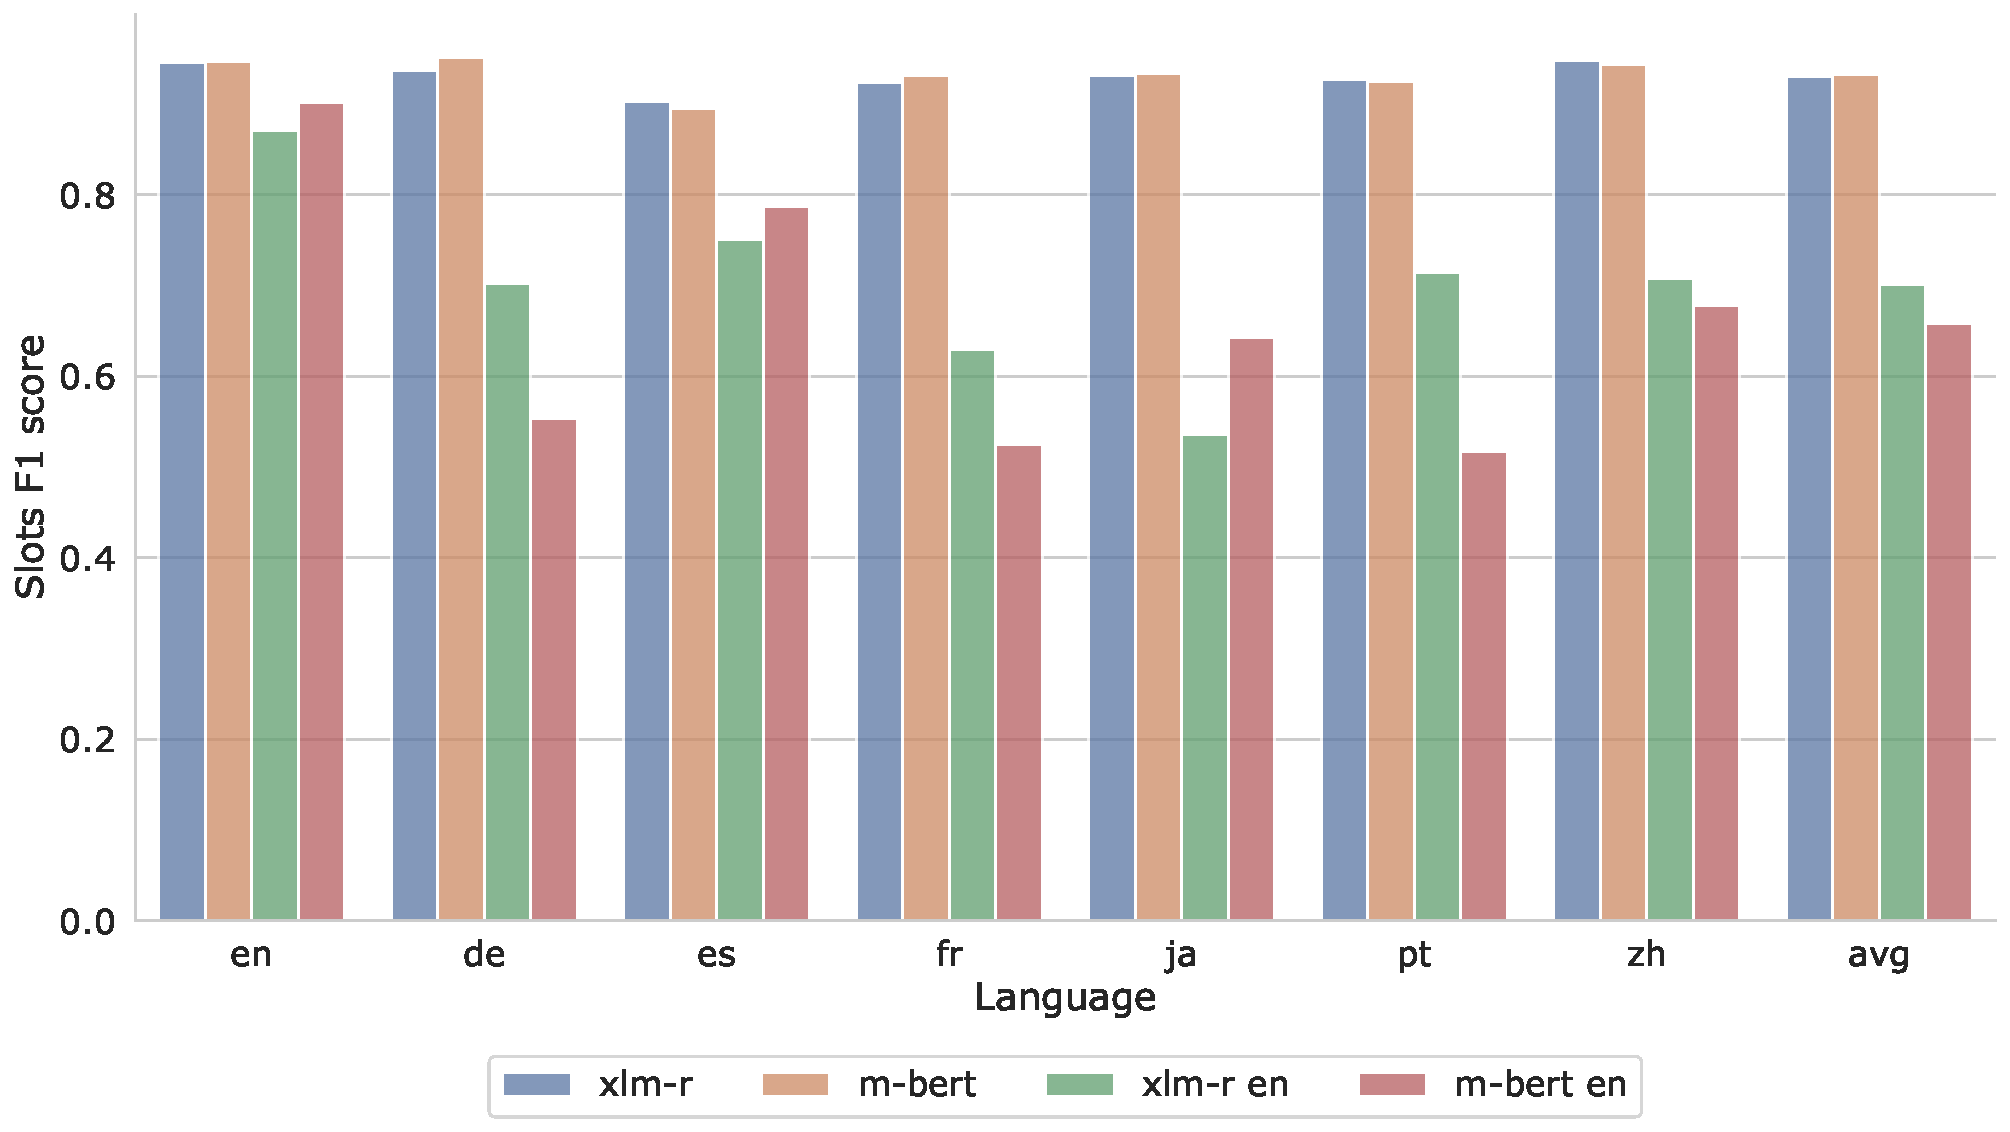
\includegraphics[width=\textwidth]{images/1}
    \caption{Сравнение моделей между собой \textbf{на тестовой выборке} датасета MultiAtis++ по метрике \textbf{Slots F1 score}.}\label{fig:figure1}
\end{figure}
\begin{figure}[h!]
    \centering
    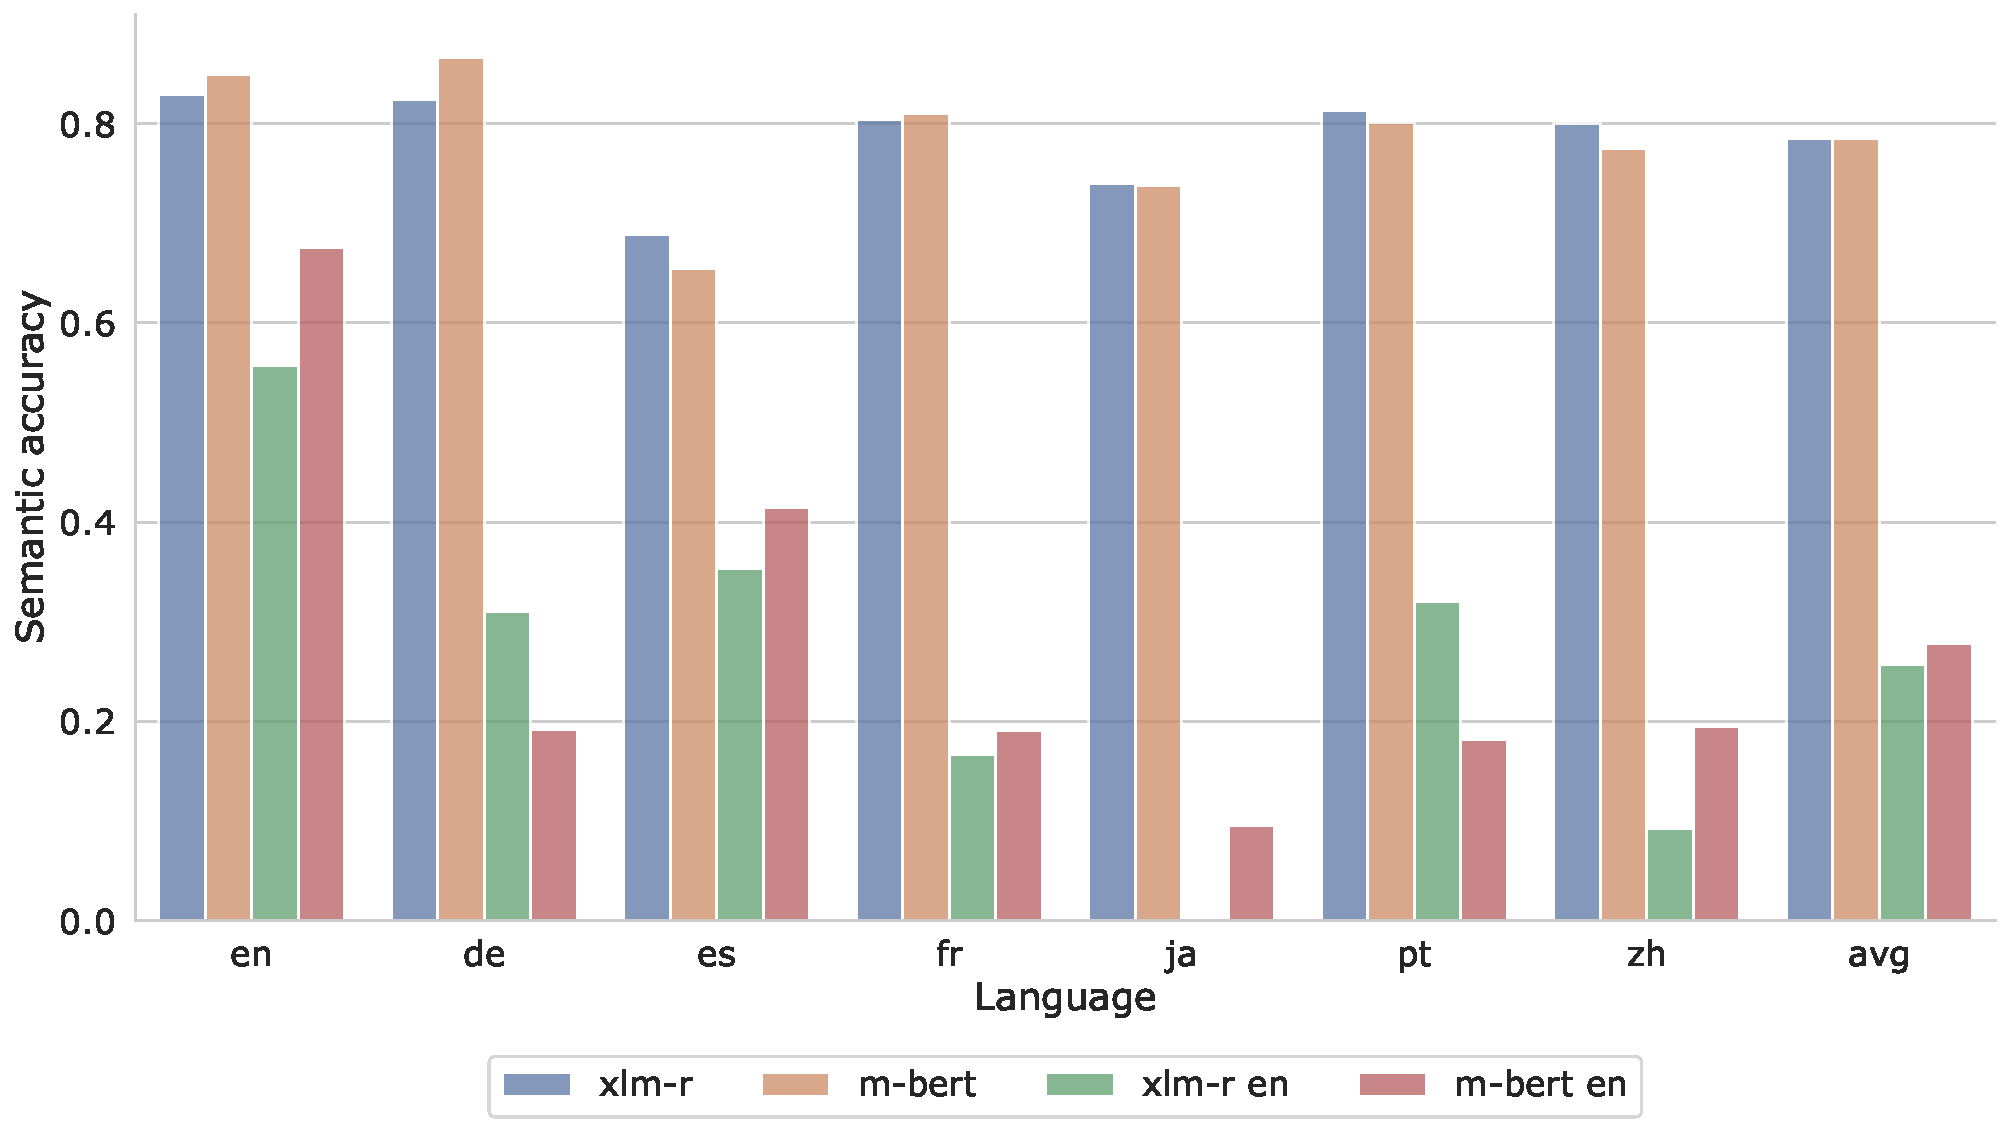
\includegraphics[width=\textwidth]{images/2}
    \caption{Сравнение моделей между собой \textbf{на тестовой выборке} датасета MultiAtis++ по метрике \textbf{Semantic accuracy}.}\label{fig:figure2}
\end{figure}

\begin{figure}[h!]
    \centering
    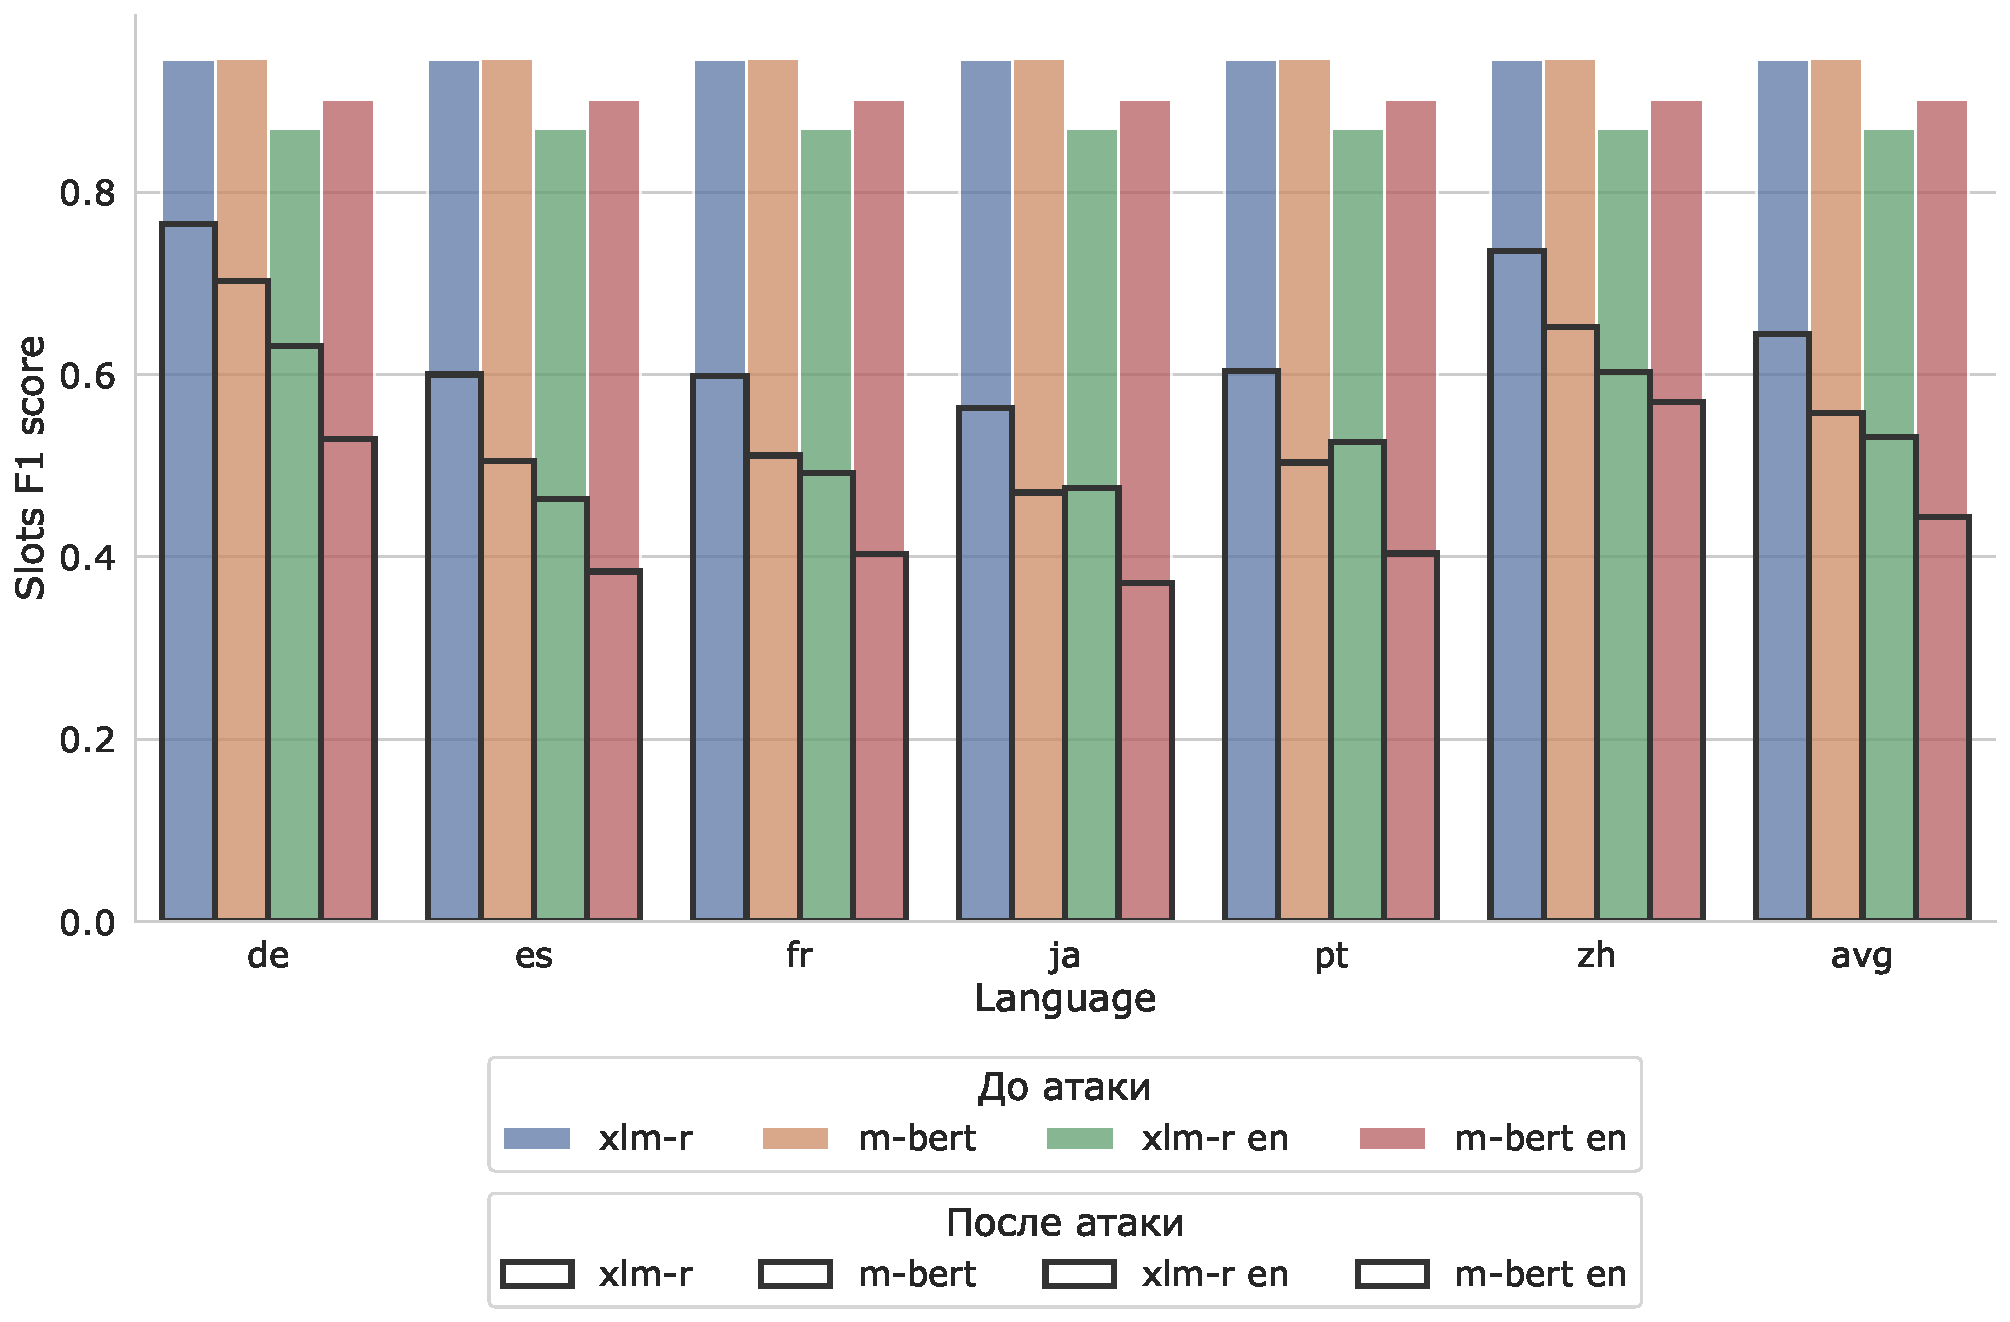
\includegraphics[width=\textwidth]{images/4}
    \caption{Сравнение моделей между собой после \textbf{word-level} атаки на тестовую выборку датасета MultiAtis++ по метрике \textbf{Slots F1 score}.}\label{fig:figure4}
\end{figure}
\begin{figure}[h!]
    \centering
    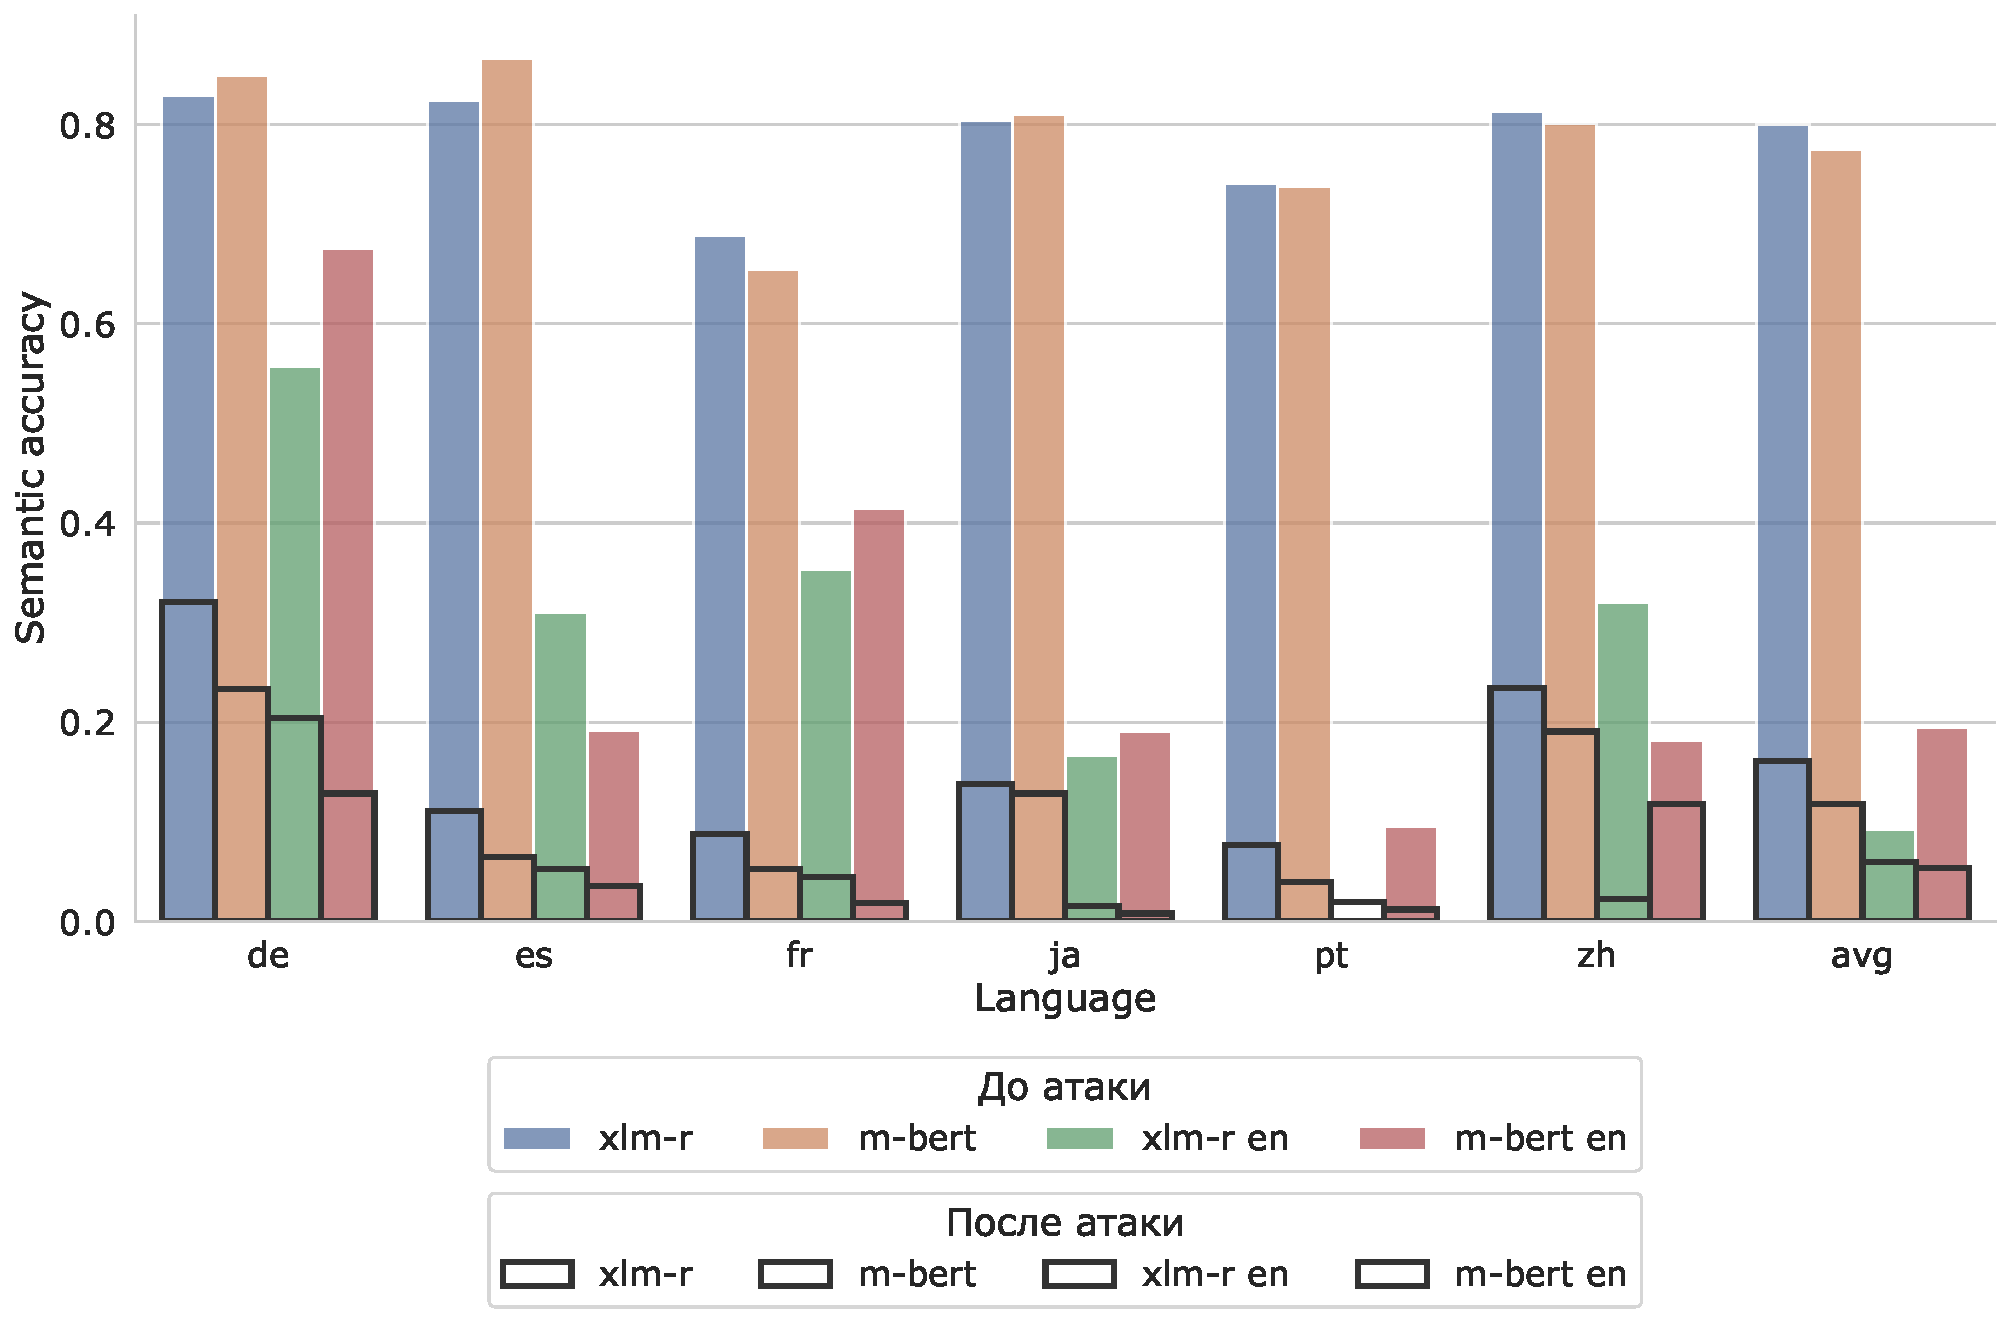
\includegraphics[width=\textwidth]{images/5}
    \caption{Сравнение моделей между собой после \textbf{word-level} атаки на тестовую выборку датасета MultiAtis++ по метрике \textbf{Semantic accuracy}.}\label{fig:figure5}
\end{figure}

\begin{figure}[h!]
    \centering
    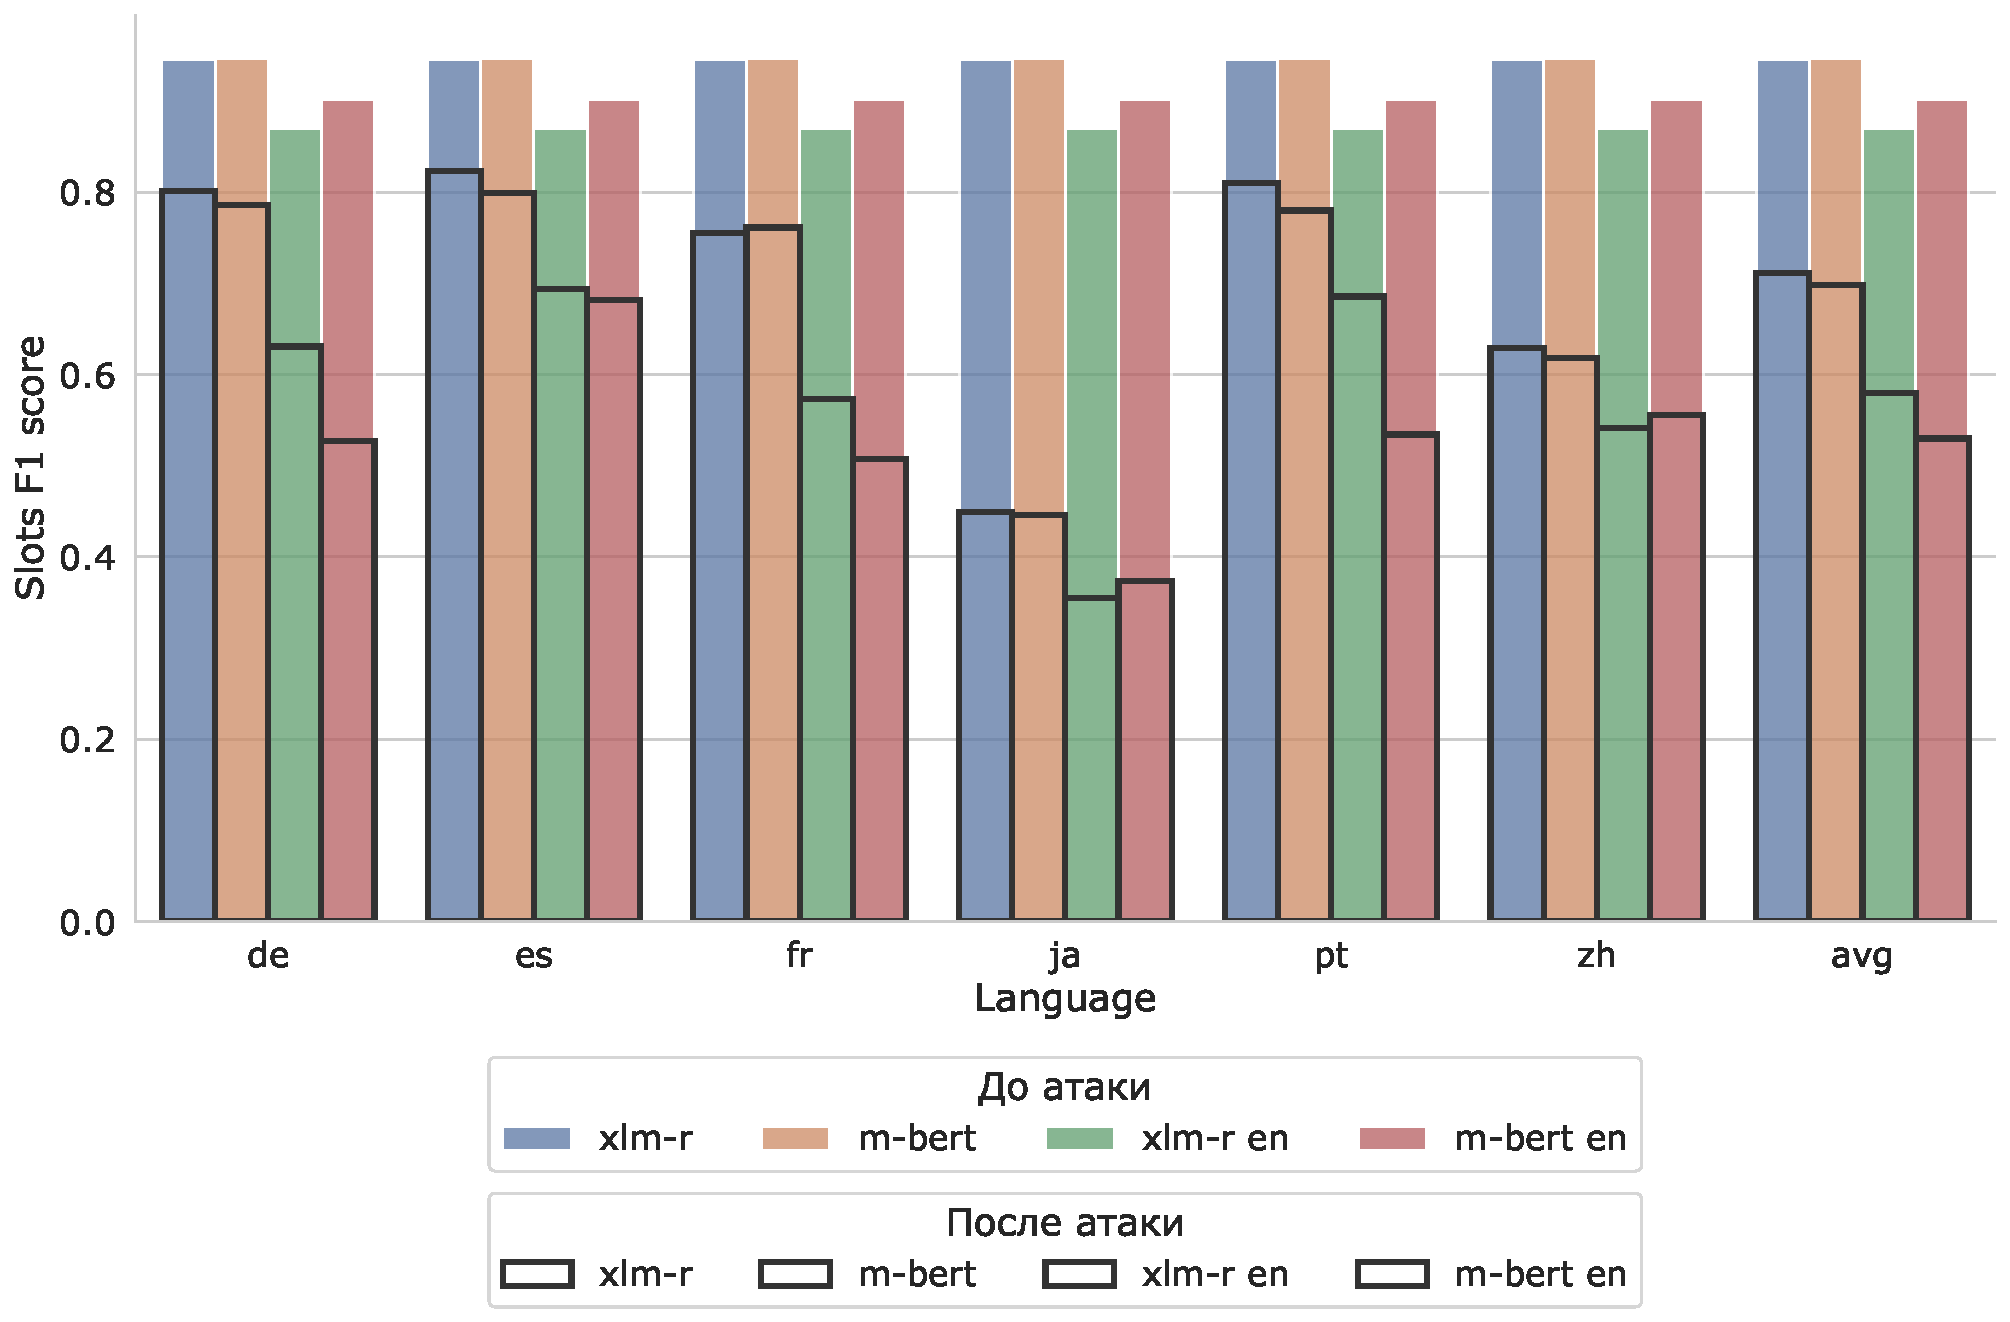
\includegraphics[width=\textwidth]{images/7}
    \caption{Сравнение моделей между собой после \textbf{phrase-level} атаки на тестовую выборку датасета MultiAtis++ по метрике \textbf{Slots F1 score}.}\label{fig:figure7}
\end{figure}
\begin{figure}[h!]
    \centering
    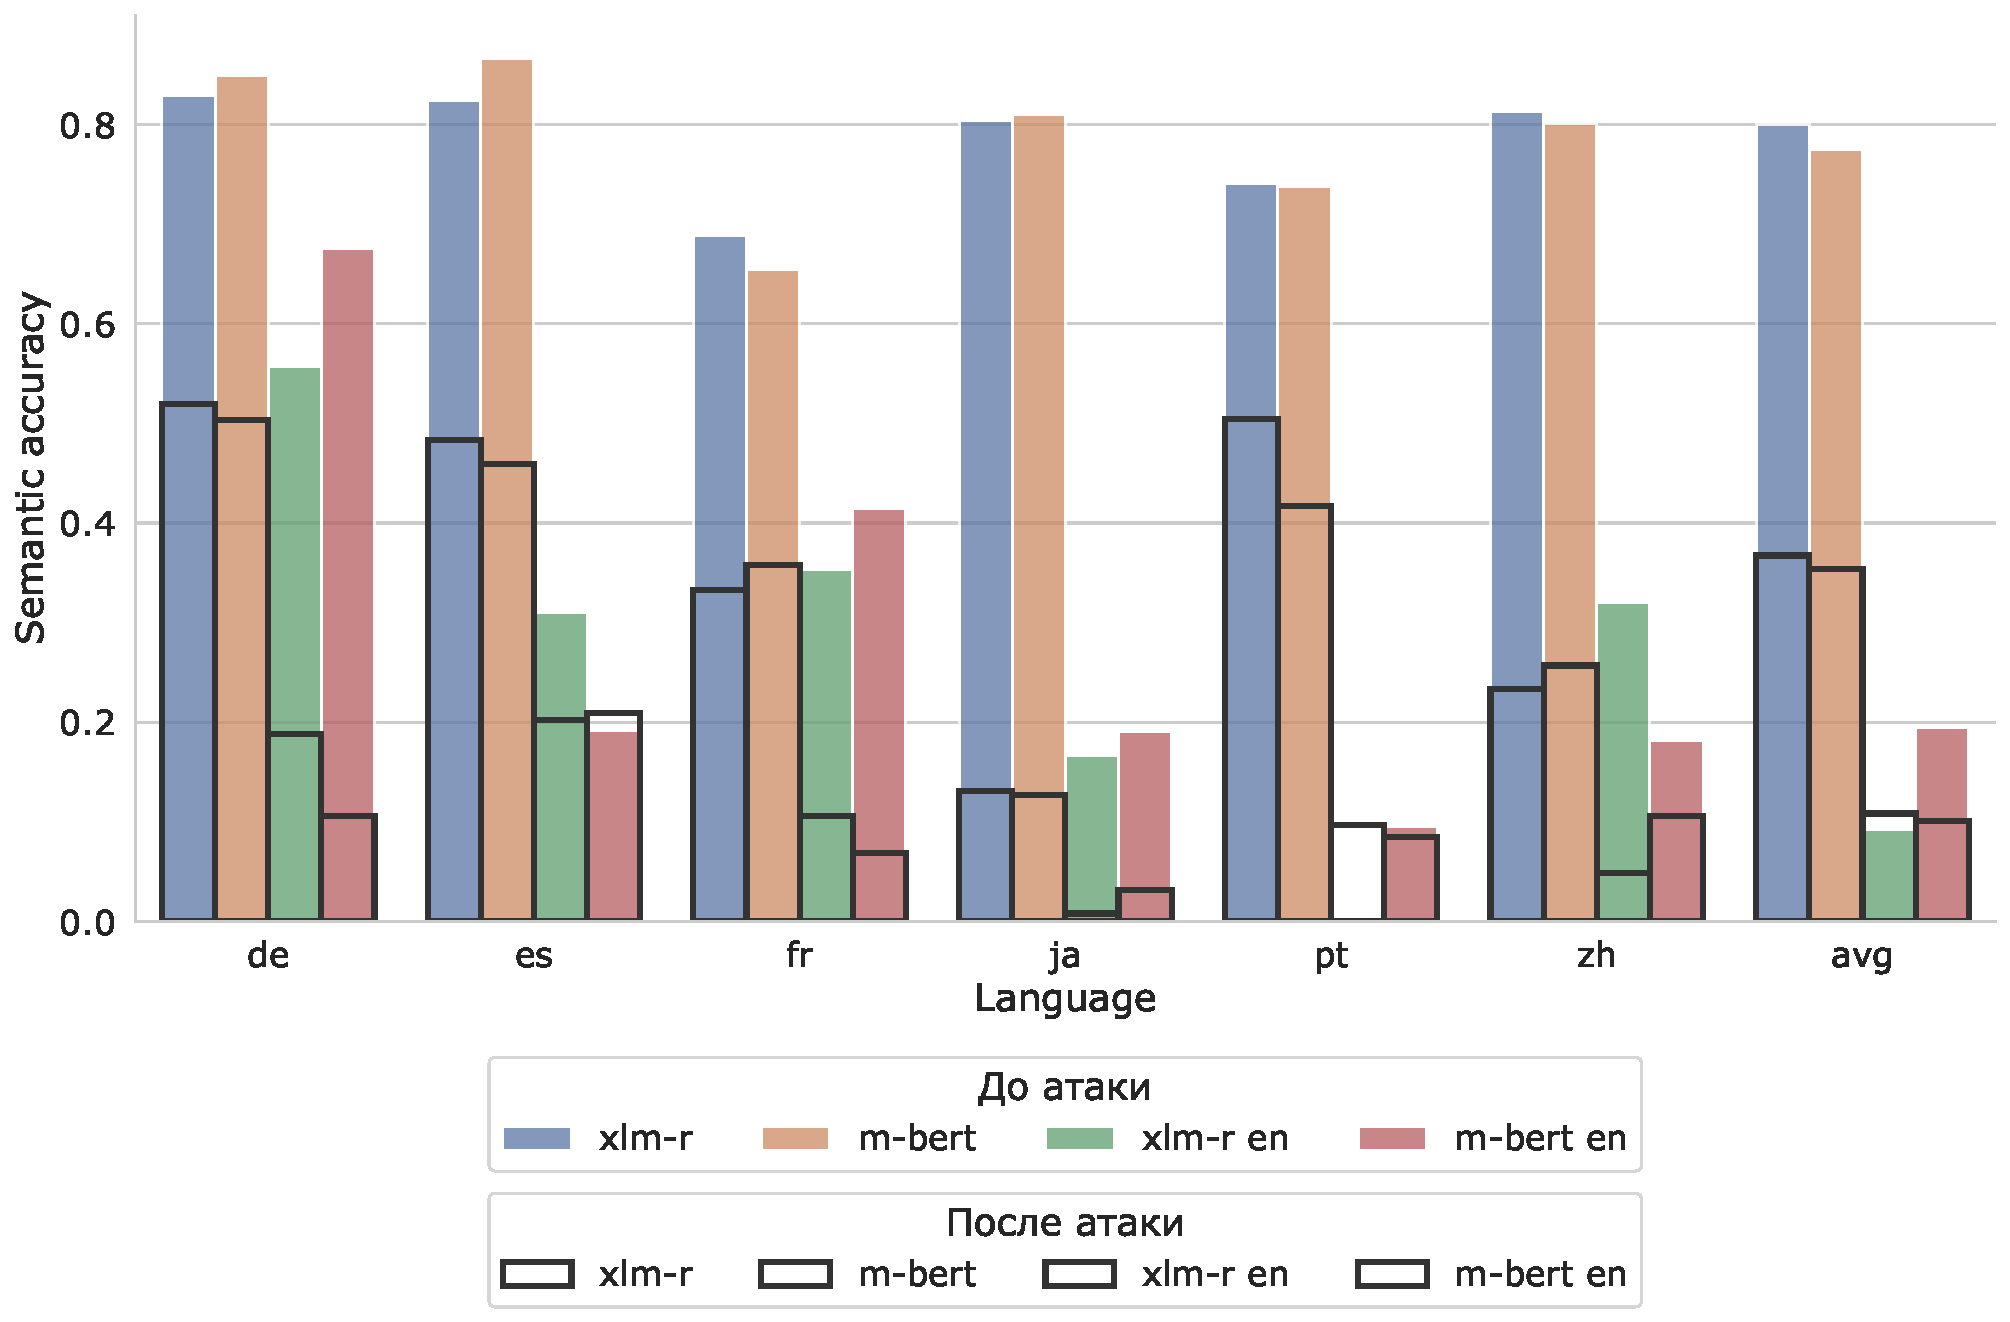
\includegraphics[width=\textwidth]{images/8}
    \caption{Сравнение моделей между собой после \textbf{phrase-level} атаки на тестовую выборку датасета MultiAtis++ по метрике \textbf{Semantic accuracy}.}\label{fig:figure8}
\end{figure}

\begin{figure}[h!]
    \centering
    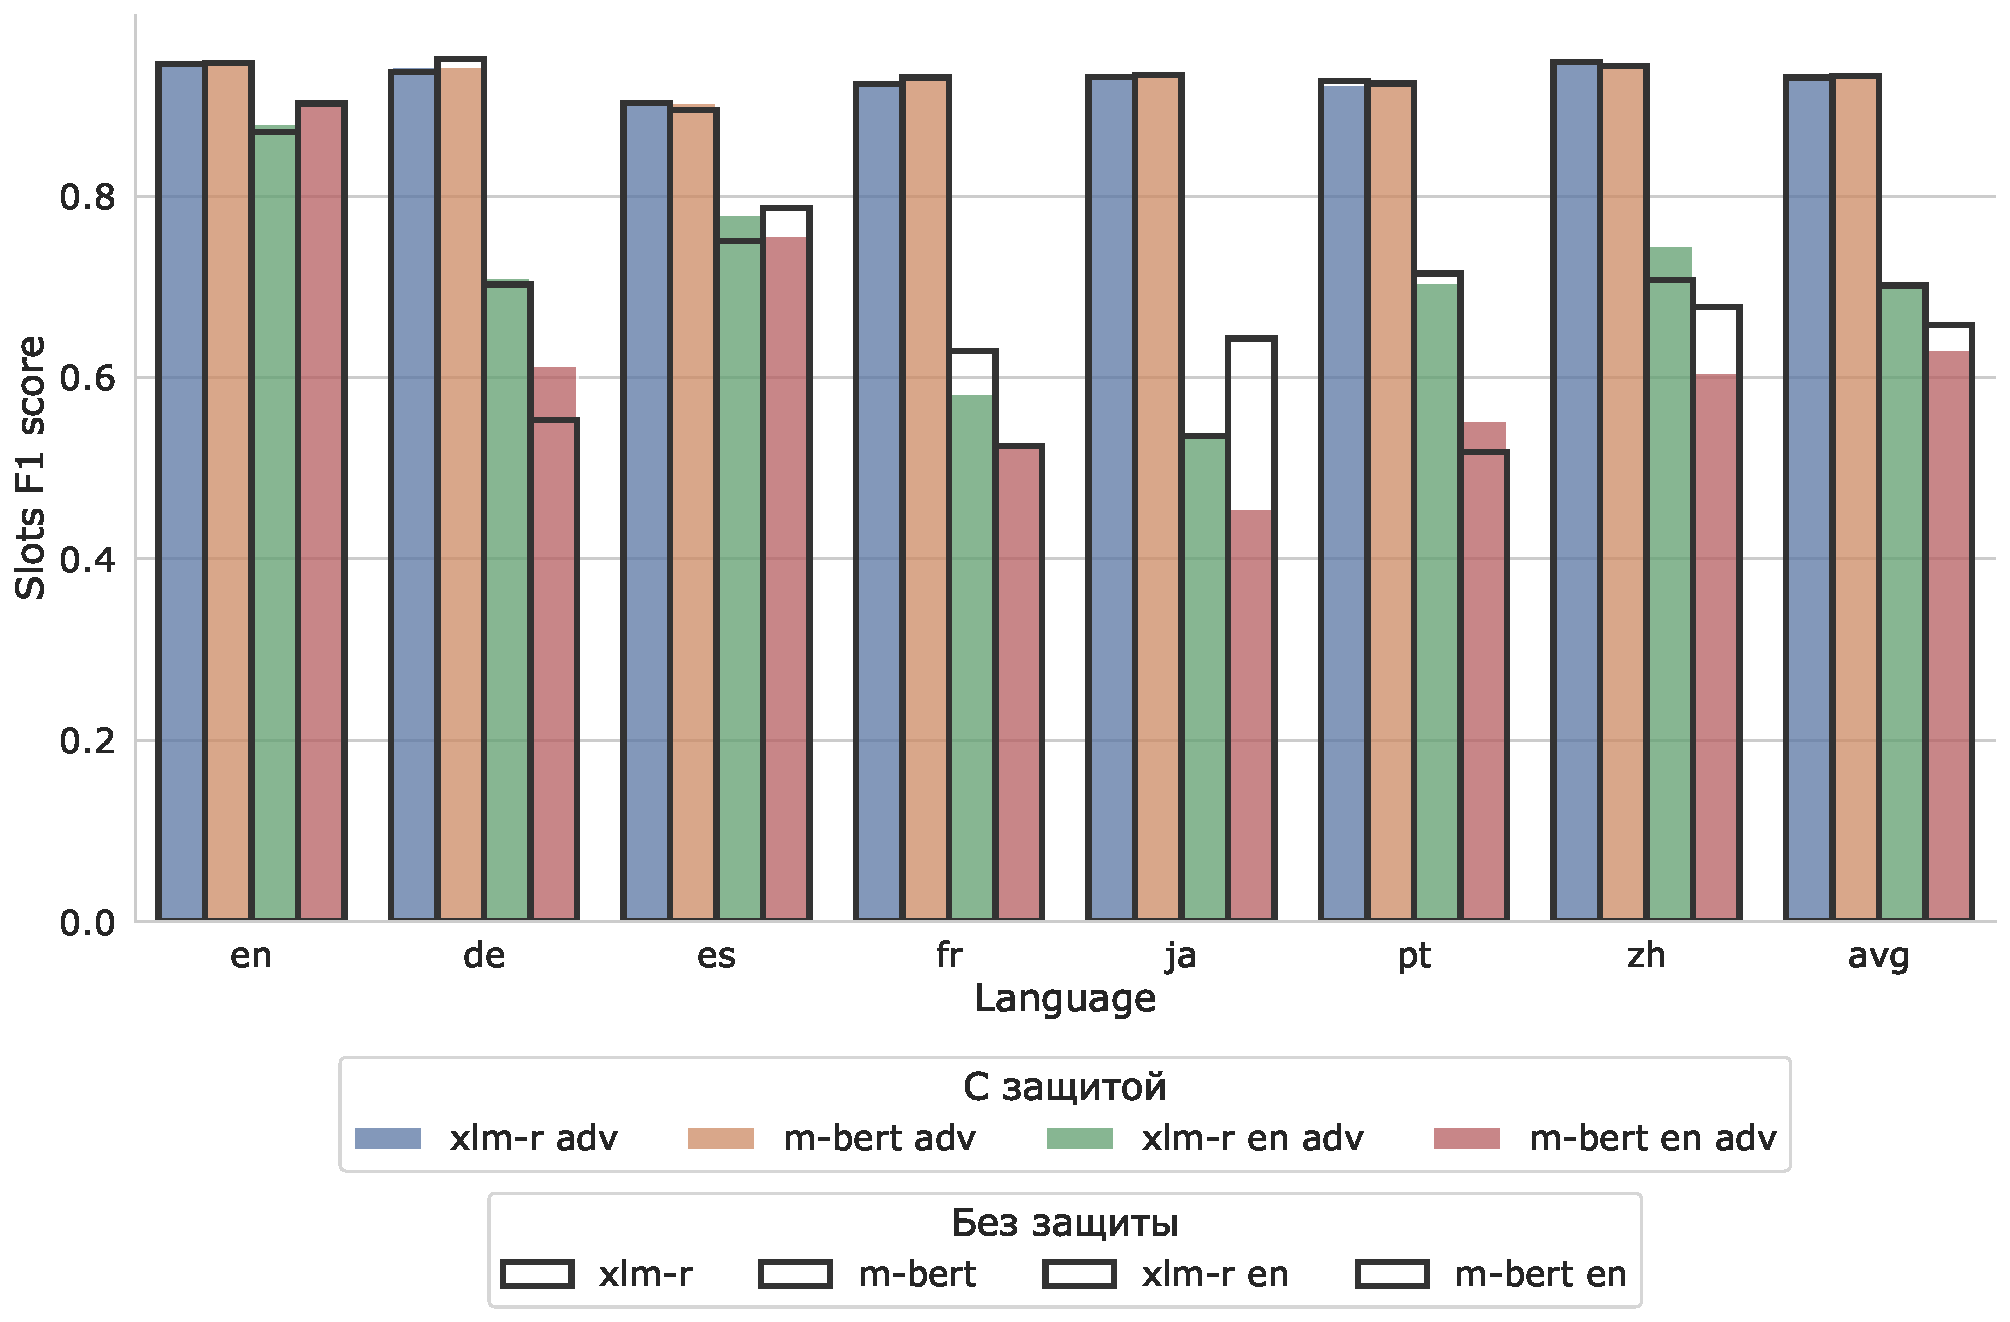
\includegraphics[width=\textwidth]{images/10}
    \caption{Сравнение моделей \textbf{с защитой} между собой \textbf{на тестовой выборке} датасета MultiAtis++ по метрике \textbf{Slots F1 score}.}\label{fig:figure10}
\end{figure}
\begin{figure}[h!]
    \centering
    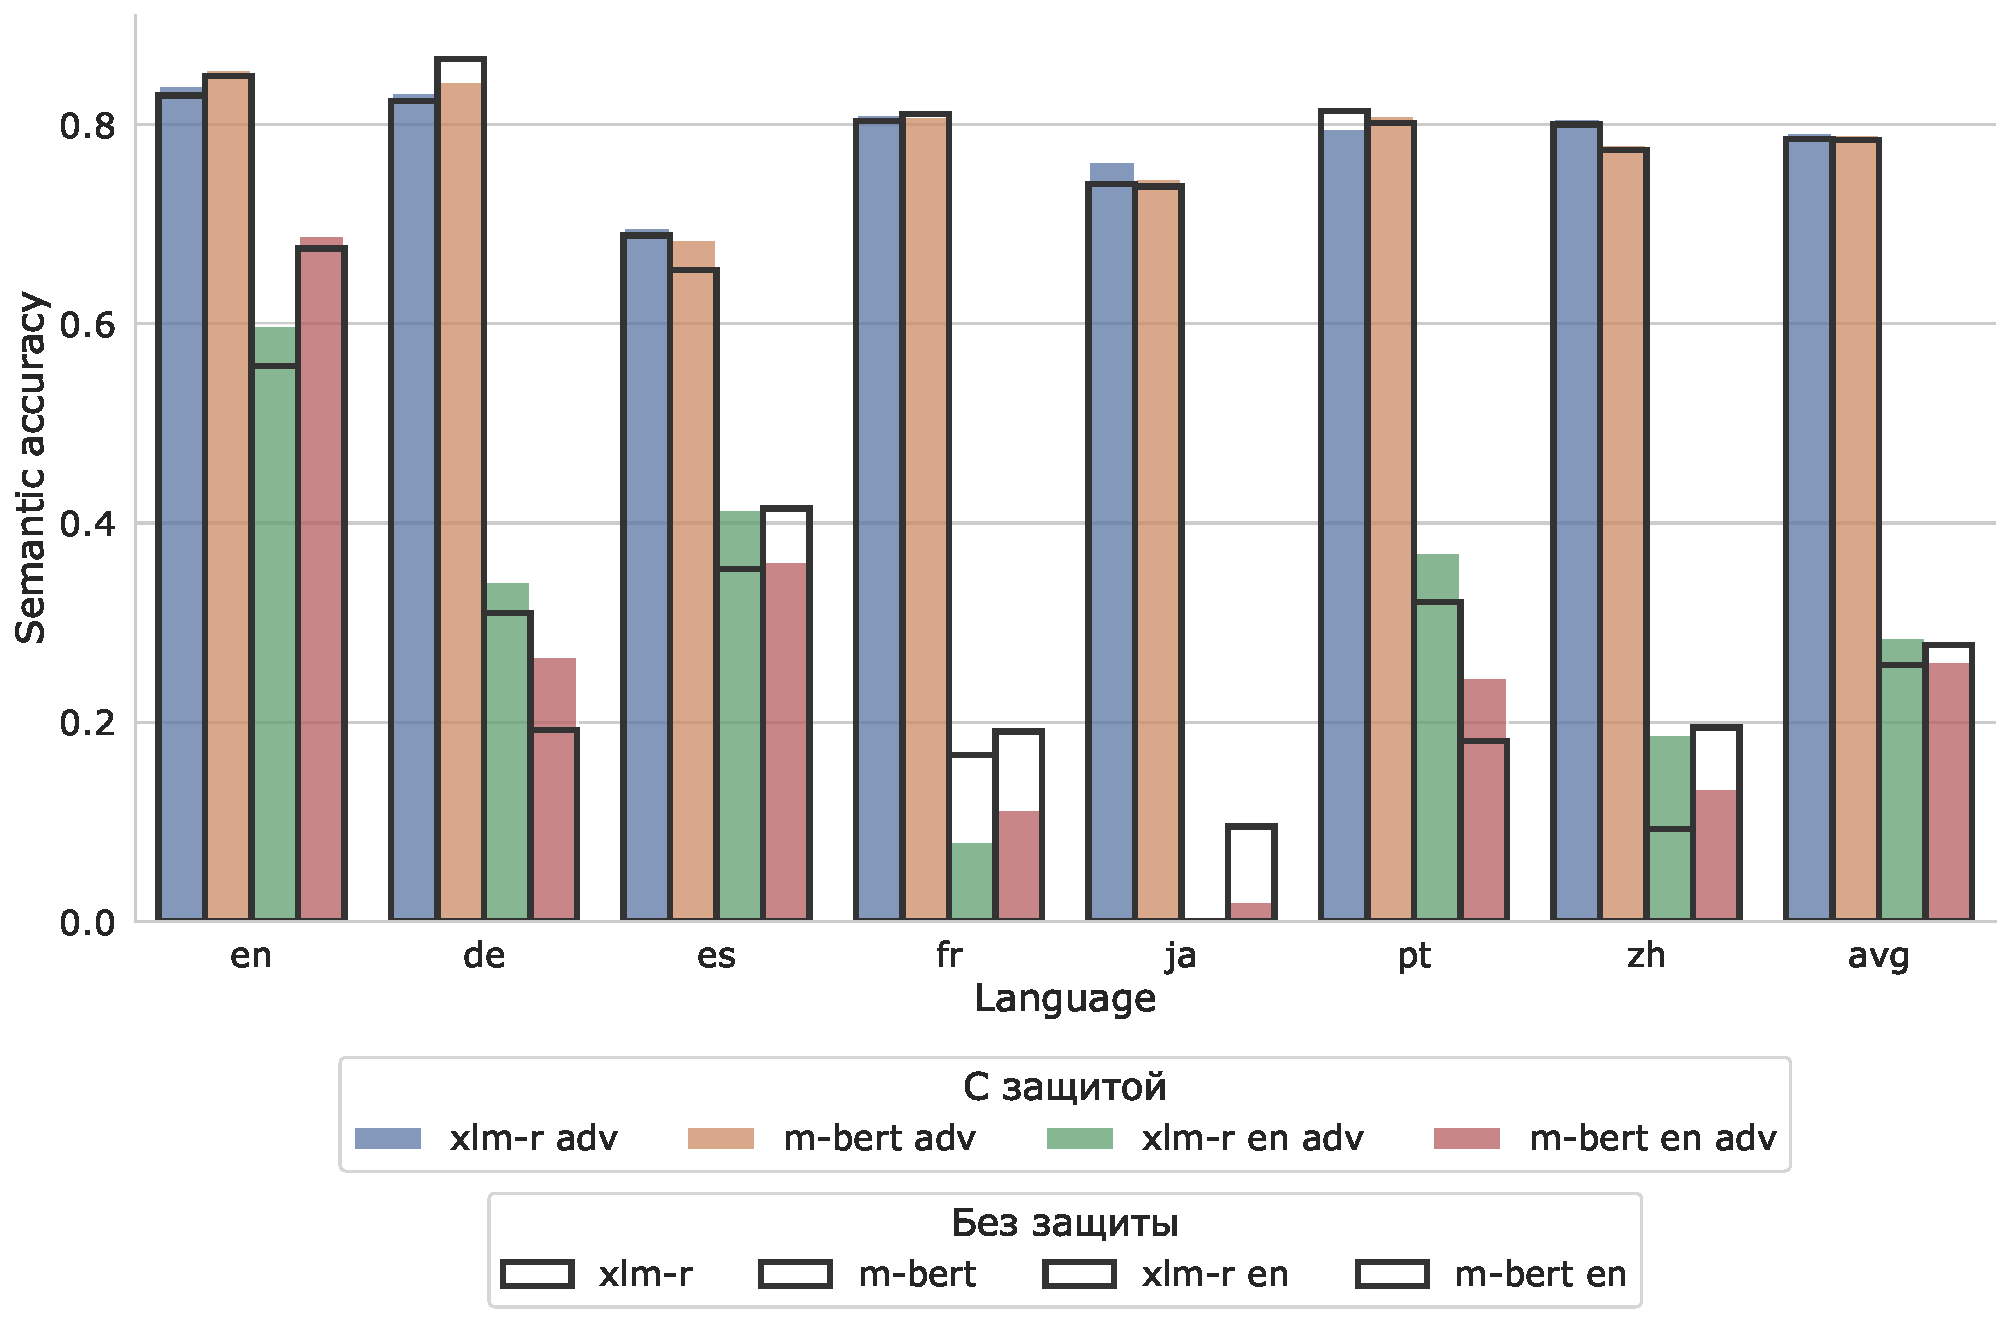
\includegraphics[width=\textwidth]{images/11}
    \caption{Сравнение моделей \textbf{с защитой} между собой \textbf{на тестовой выборке} датасета MultiAtis++ по метрике \textbf{Semantic accuracy}.}\label{fig:figure11}
\end{figure}

\begin{figure}[h!]
    \centering
    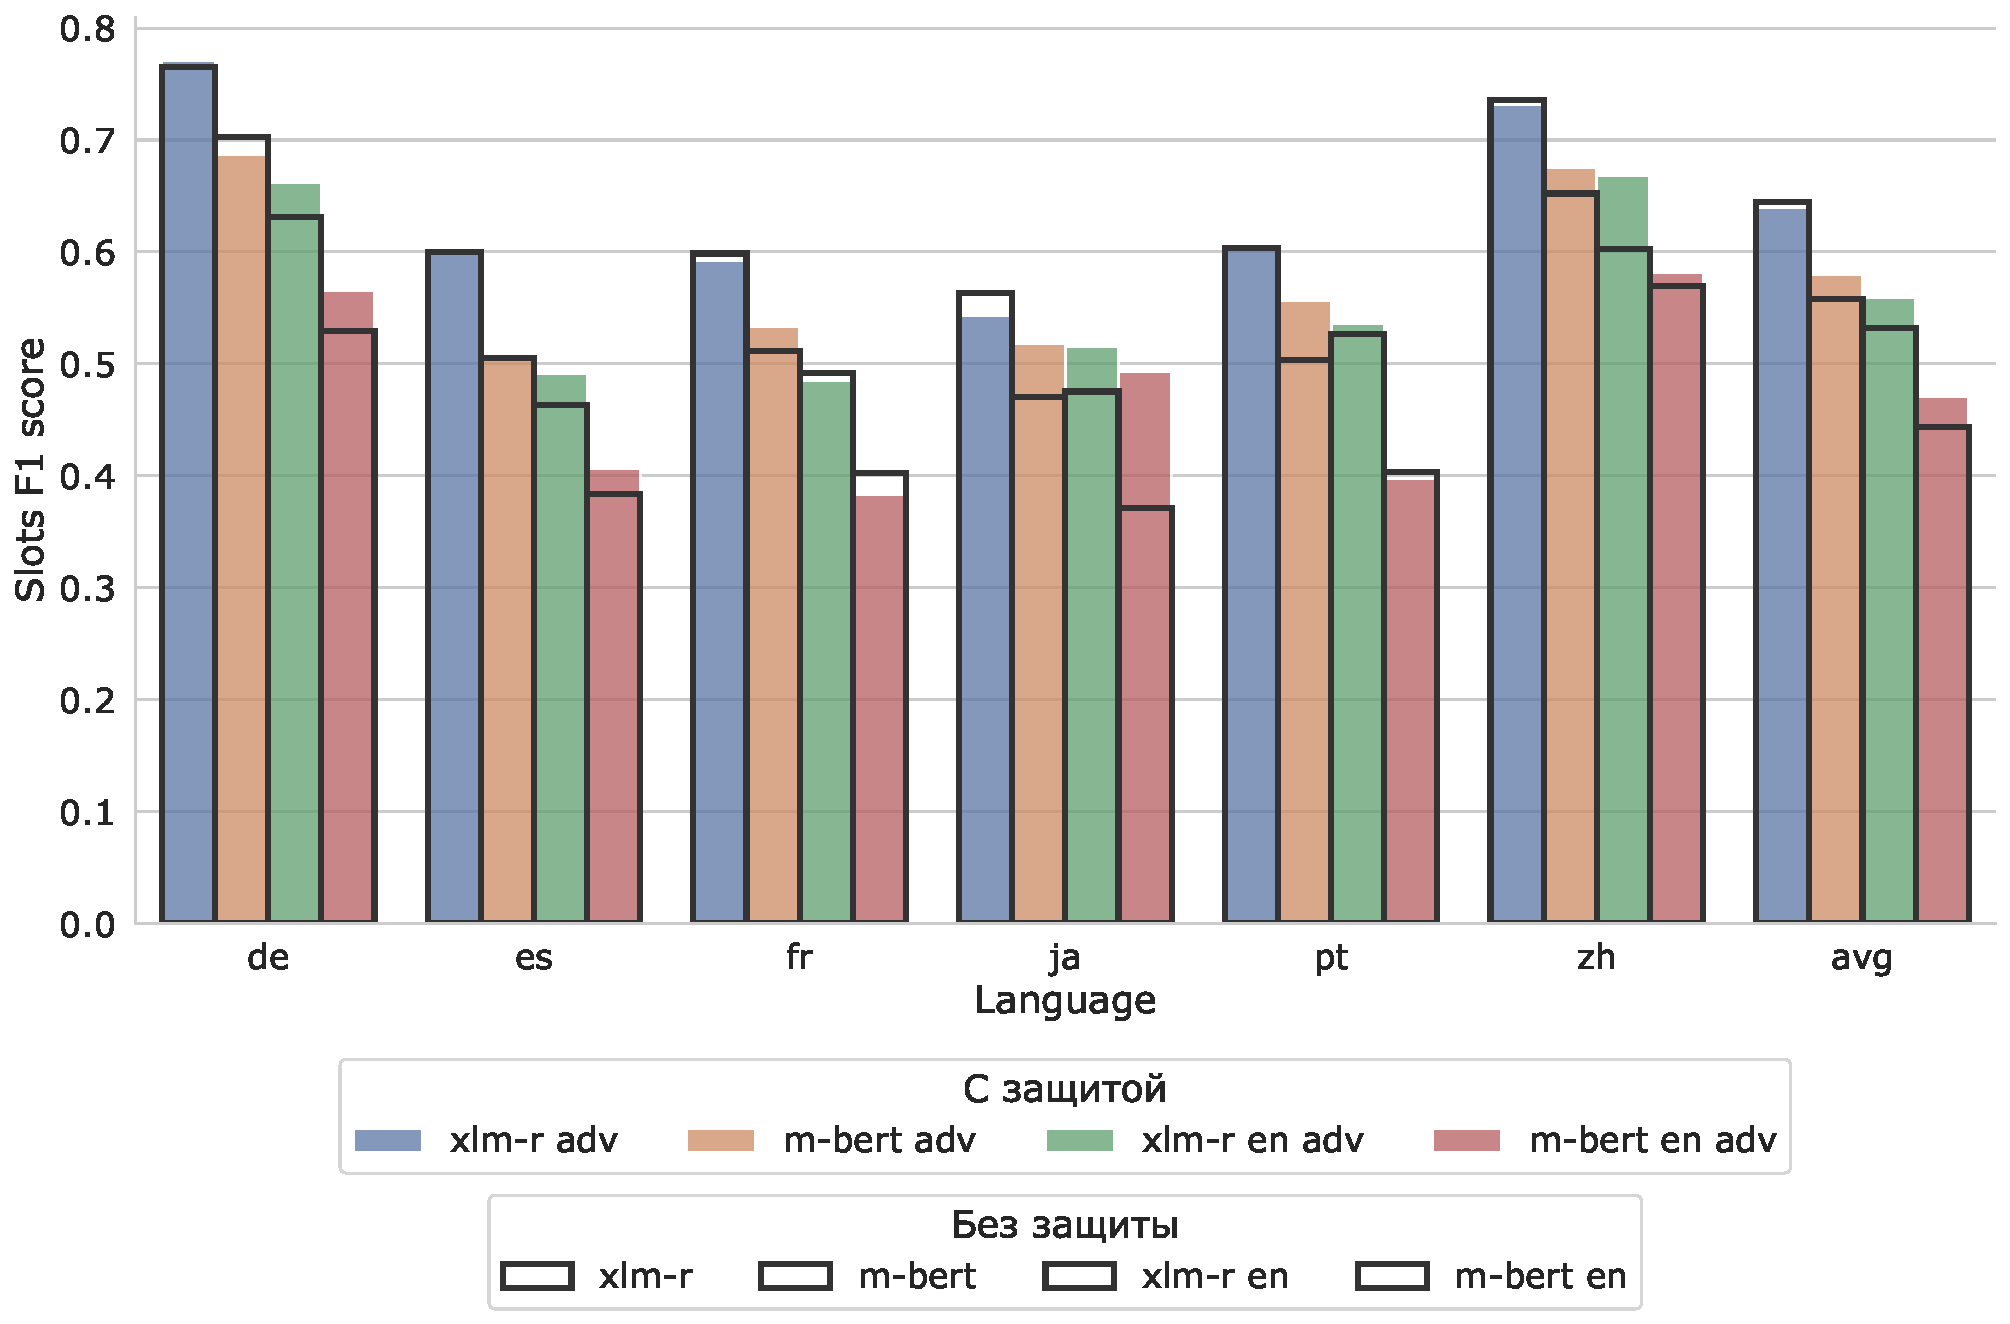
\includegraphics[width=\textwidth]{images/13}
    \caption{Сравнение моделей \textbf{с защитой} между собой после \textbf{word-level} атаки на тестовую выборку датасета MultiAtis++ по метрике \textbf{Slots F1 score}.}\label{fig:figure13}
\end{figure}
\begin{figure}[h!]
    \centering
    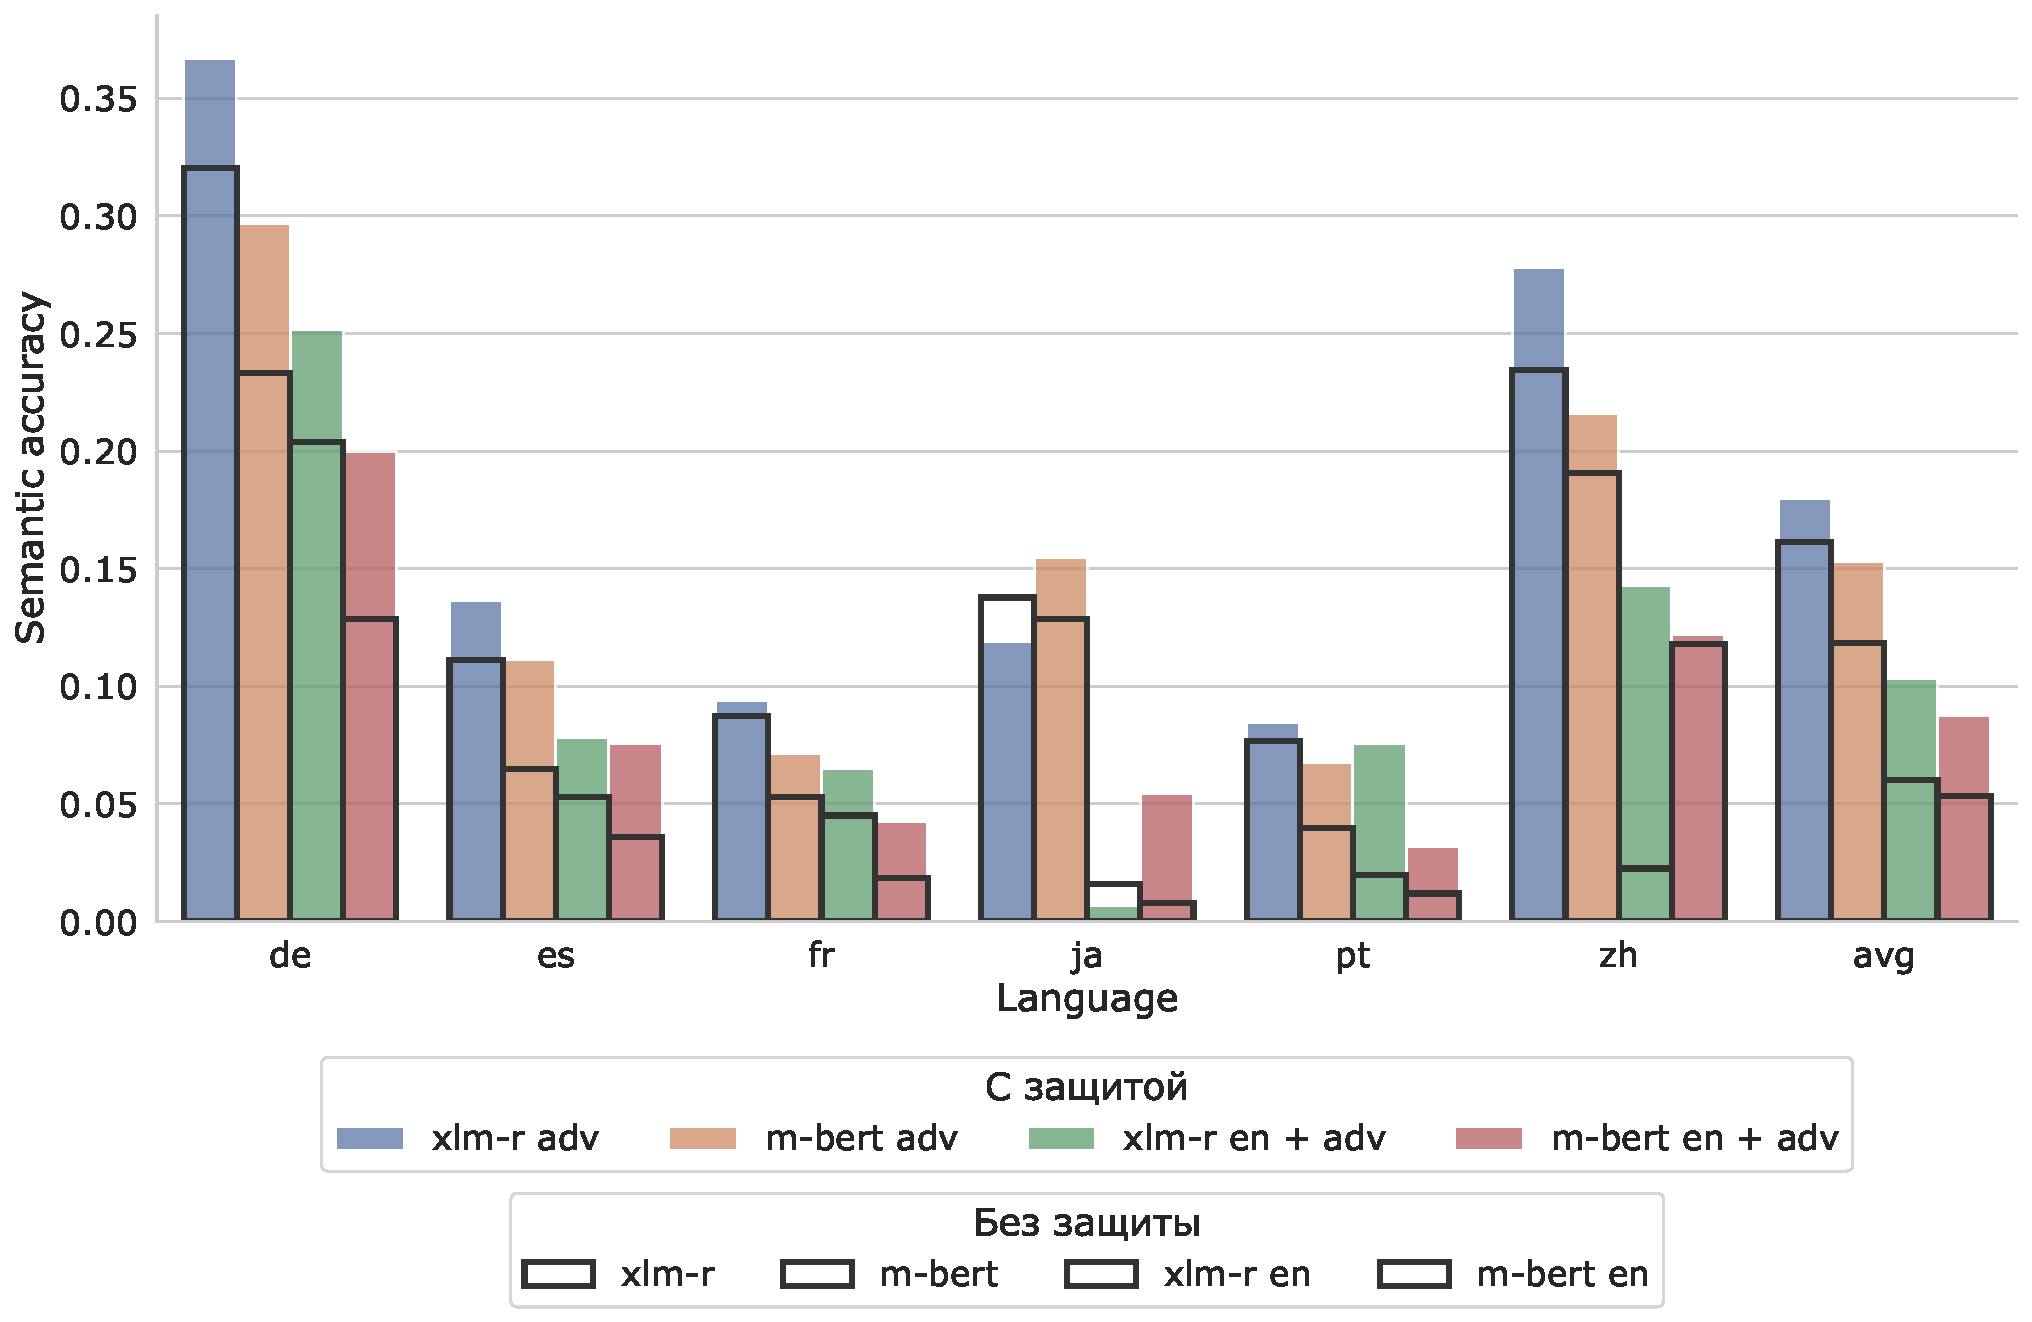
\includegraphics[width=\textwidth]{images/14}
    \caption{Сравнение моделей \textbf{с защитой} между собой после \textbf{word-level} атаки на тестовую выборку датасета MultiAtis++ по метрике \textbf{Semantic accuracy}.}\label{fig:figure14}
\end{figure}

\begin{figure}[h!]
    \centering
    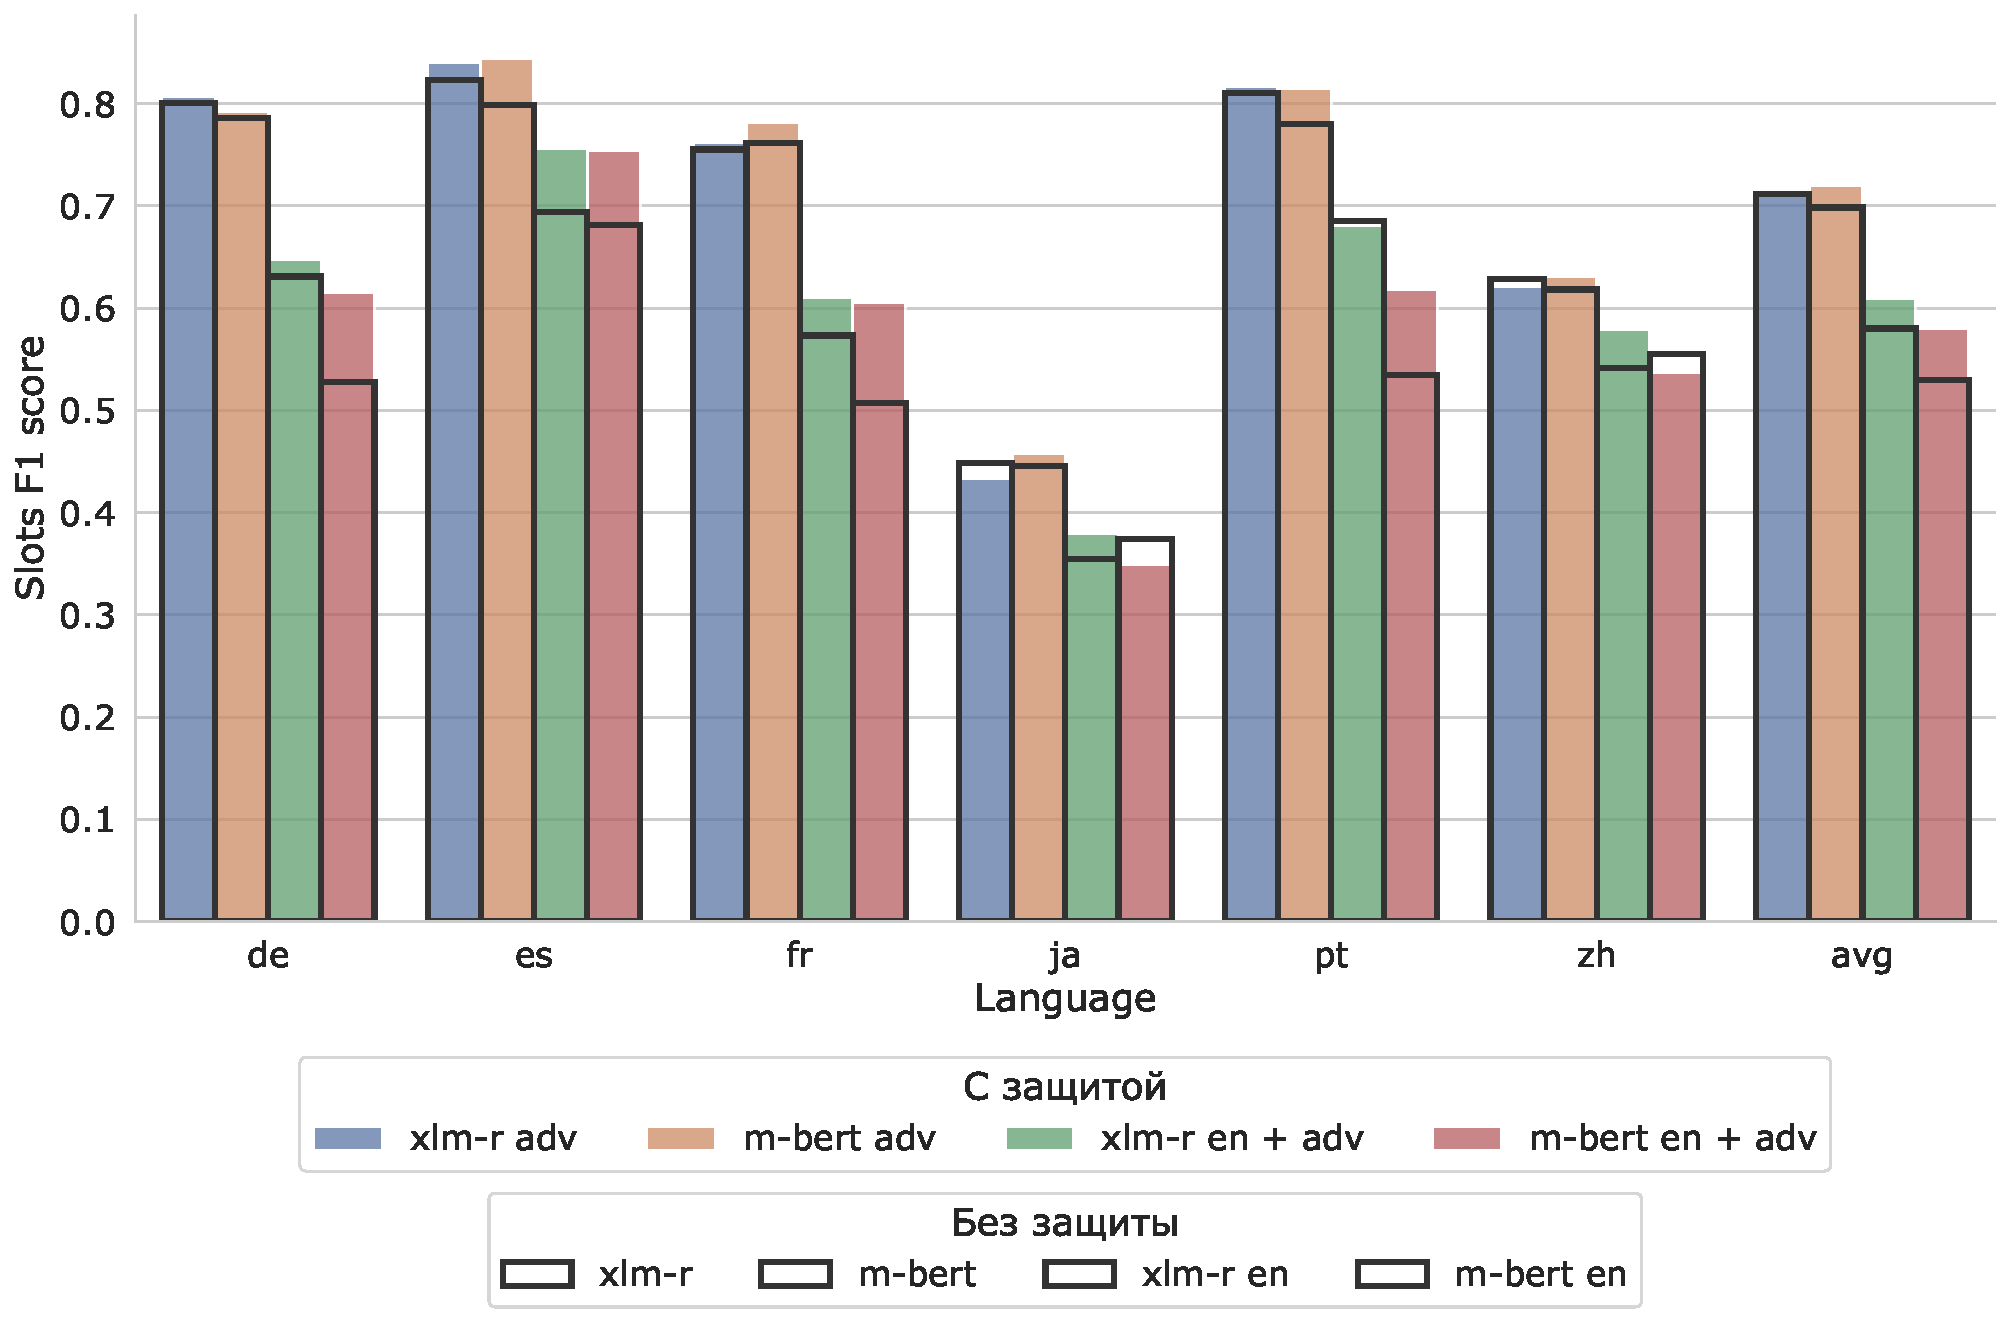
\includegraphics[width=\textwidth]{images/16}
    \caption{Сравнение моделей \textbf{с защитой} между собой после \textbf{phrase-level} атаки на тестовую выборку датасета MultiAtis++ по метрике \textbf{Slots F1 score}.}\label{fig:figure16}
\end{figure}
\begin{figure}[h!]
    \centering
    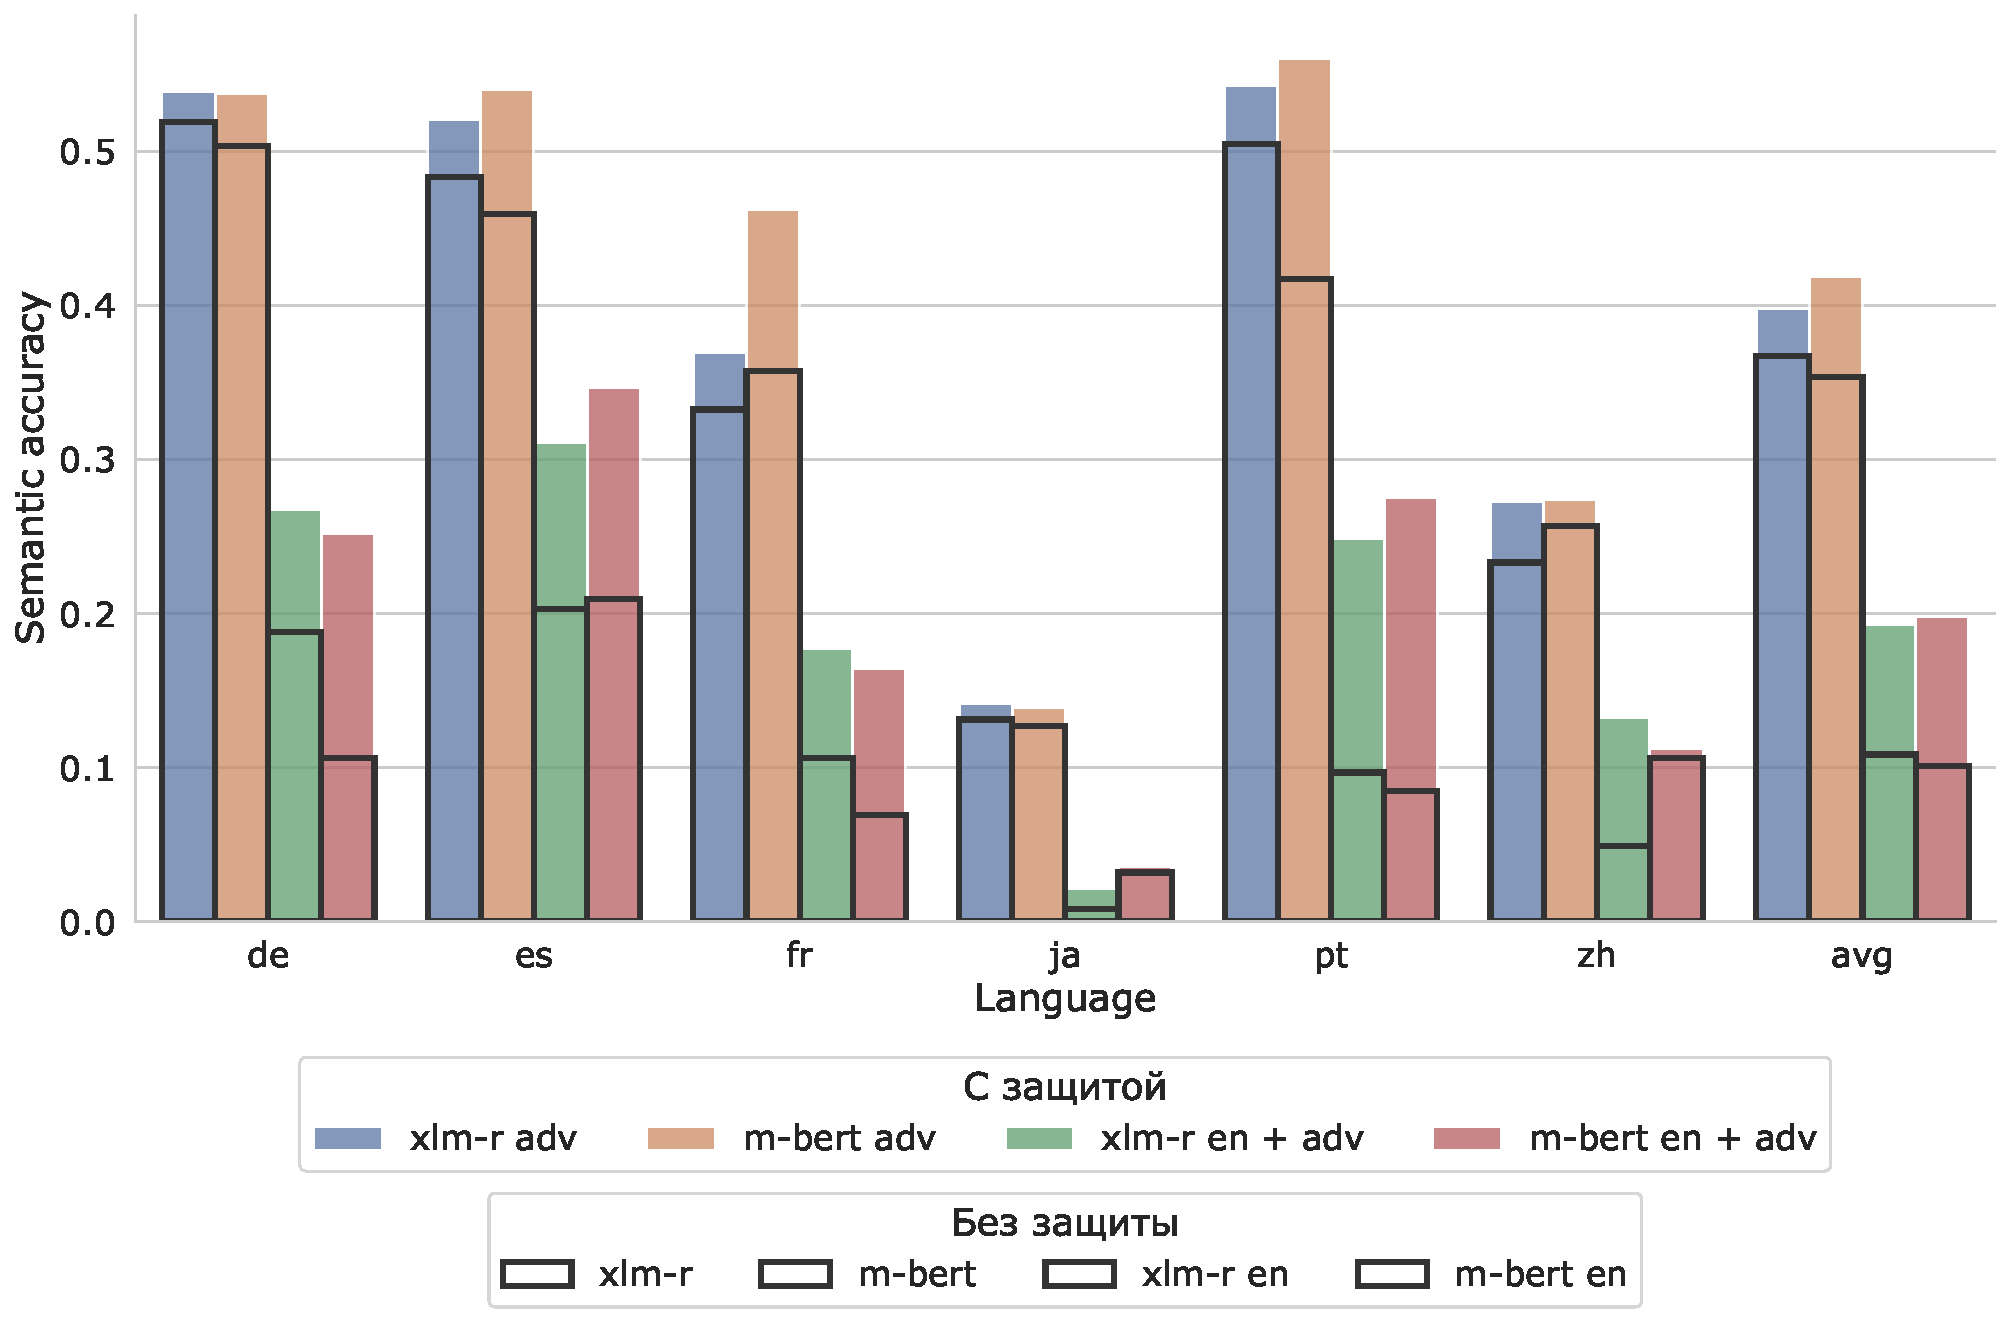
\includegraphics[width=\textwidth]{images/17}
    \caption{Сравнение моделей \textbf{с защитой} между собой после \textbf{phrase-level} атаки на тестовую выборку датасета MultiAtis++ по метрике \textbf{Semantic accuracy}.}\label{fig:figure17}
\end{figure}

\subsection*{Г. Таблицы с результатами экспериментов}
\addcontentsline{toc}{subsection}{Г. Таблицы с результатами экспериментов}

\begin{table}[H]
	\resizebox{\textwidth}{!}{
		\begin{tabular}{|>{\bfseries}l|c|c|c|c|c|c|c|c|}
			\hline
			& en & de & es & fr & ja & pt & zh & avg \\ \hline
			xlm-r&$0.980$ & $0.975$ & $0.968$ & $0.972$ & $0.977$ & $0.970$ & $0.968$ & $0.973$ \\ \hline
			m-bert&$0.977$ & $0.977$ & $0.963$ & $0.966$ & $0.959$ & $0.967$ & $0.962$ & $0.967$ \\ \hline
			xlm-r en&$0.903$ & $0.885$ & $0.882$ & $0.879$ & $0.830$ & $0.846$ & $0.856$ & $0.869$ \\ \hline
			m-bert en&$0.951$ & $0.828$ & $0.865$ & $0.877$ & $0.750$ & $0.853$ & $0.795$ & $0.845$ \\ \hline
		\end{tabular}
	}\caption{Сравнение моделей между собой \textbf{на тестовой выборке} датасета MultiAtis++ по метрике \textbf{Intent accuracy}. По колонкам языки тестовых подвыборок, по рядам тестируемые модели.}\label{tab:table0}
\end{table}
\begin{table}[H]
	\resizebox{\textwidth}{!}{
		\begin{tabular}{|>{\bfseries}l|c|c|c|c|c|c|c|c|}
			\hline
			& en & de & es & fr & ja & pt & zh & avg \\ \hline
			xlm-r&$0.945$ & $0.937$ & $0.902$ & $0.924$ & $0.931$ & $0.927$ & $0.948$ & $0.931$ \\ \hline
			m-bert&$0.947$ & $0.951$ & $0.895$ & $0.931$ & $0.933$ & $0.924$ & $0.944$ & $0.932$ \\ \hline
			xlm-r en&$0.871$ & $0.702$ & $0.750$ & $0.629$ & $0.535$ & $0.715$ & $0.707$ & $0.701$ \\ \hline
			m-bert en&$0.902$ & $0.553$ & $0.787$ & $0.524$ & $0.643$ & $0.517$ & $0.678$ & $0.658$ \\ \hline
		\end{tabular}
	}\caption{Сравнение моделей между собой \textbf{на тестовой выборке} датасета MultiAtis++ по метрике \textbf{Slots F1 score}. По колонкам языки тестовых подвыборок, по рядам тестируемые модели.}\label{tab:table1}
\end{table}
\begin{table}[H]
	\resizebox{\textwidth}{!}{
		\begin{tabular}{|>{\bfseries}l|c|c|c|c|c|c|c|c|}
			\hline
			& en & de & es & fr & ja & pt & zh & avg \\ \hline
			xlm-r&$0.829$ & $0.824$ & $0.689$ & $0.804$ & $0.740$ & $0.813$ & $0.800$ & $0.786$ \\ \hline
			m-bert&$0.849$ & $0.866$ & $0.654$ & $0.811$ & $0.738$ & $0.801$ & $0.775$ & $0.785$ \\ \hline
			xlm-r en&$0.558$ & $0.310$ & $0.354$ & $0.167$ & $0.000$ & $0.321$ & $0.093$ & $0.257$ \\ \hline
			m-bert en&$0.675$ & $0.192$ & $0.415$ & $0.191$ & $0.095$ & $0.181$ & $0.195$ & $0.278$ \\ \hline
		\end{tabular}
	}\caption{Сравнение моделей между собой \textbf{на тестовой выборке} датасета MultiAtis++ по метрике \textbf{Semantic accuracy}. По колонкам языки тестовых подвыборок, по рядам тестируемые модели.}\label{tab:table2}
\end{table}

\begin{table}[H]
	\resizebox{\textwidth}{!}{
		\begin{tabular}{|>{\bfseries}l|c|c|c|c|c|c|c|}
			\hline
			& de & es & fr & ja & pt & zh & avg \\ \hline
			xlm-r&$0.931$ & $0.877$ & $0.849$ & $0.825$ & $0.901$ & $0.872$ & $0.876$ \\ \hline
			m-bert&$0.893$ & $0.891$ & $0.872$ & $0.820$ & $0.853$ & $0.852$ & $0.863$ \\ \hline
			xlm-r en&$0.809$ & $0.783$ & $0.774$ & $0.677$ & $0.554$ & $0.728$ & $0.721$ \\ \hline
			m-bert en&$0.811$ & $0.760$ & $0.793$ & $0.723$ & $0.760$ & $0.777$ & $0.771$ \\ \hline
		\end{tabular}
	}\caption{Сравнение моделей между собой после word-level атаки на тестовую выборку датасета MultiAtis++ по метрике \textbf{Intent accuracy}. По колонкам встраиваемые языки, по рядам тестируемые модели.}\label{tab:table3}
\end{table}
\begin{table}[H]
	\resizebox{\textwidth}{!}{
		\begin{tabular}{|>{\bfseries}l|c|c|c|c|c|c|c|}
			\hline
			& de & es & fr & ja & pt & zh & avg \\ \hline
			xlm-r&$0.767$ & $0.589$ & $0.603$ & $0.552$ & $0.598$ & $0.747$ & $0.642$ \\ \hline
			m-bert&$0.685$ & $0.517$ & $0.510$ & $0.428$ & $0.494$ & $0.684$ & $0.553$ \\ \hline
			xlm-r en&$0.642$ & $0.467$ & $0.499$ & $0.508$ & $0.543$ & $0.641$ & $0.550$ \\ \hline
			m-bert en&$0.539$ & $0.385$ & $0.419$ & $0.362$ & $0.391$ & $0.585$ & $0.447$ \\ \hline
		\end{tabular}
	}\caption{Сравнение моделей между собой после word-level атаки на тестовую выборку датасета MultiAtis++ по метрике \textbf{Slots F1 score}. По колонкам встраиваемые языки, по рядам тестируемые модели.}\label{tab:table4}
\end{table}
\begin{table}[H]
	\resizebox{\textwidth}{!}{
		\begin{tabular}{|>{\bfseries}l|c|c|c|c|c|c|c|}
			\hline
			& de & es & fr & ja & pt & zh & avg \\ \hline
			xlm-r&$0.343$ & $0.109$ & $0.086$ & $0.170$ & $0.077$ & $0.278$ & $0.177$ \\ \hline
			m-bert&$0.228$ & $0.083$ & $0.058$ & $0.081$ & $0.038$ & $0.213$ & $0.117$ \\ \hline
			xlm-r en&$0.201$ & $0.057$ & $0.056$ & $0.013$ & $0.023$ & $0.042$ & $0.065$ \\ \hline
			m-bert en&$0.136$ & $0.029$ & $0.032$ & $0.005$ & $0.011$ & $0.115$ & $0.055$ \\ \hline
		\end{tabular}
	}\caption{Сравнение моделей между собой после word-level атаки на тестовую выборку датасета MultiAtis++ по метрике \textbf{Semantic accuracy}. По колонкам встраиваемые языки, по рядам тестируемые модели.}\label{tab:table5}
\end{table}

\begin{table}[H]
	\resizebox{\textwidth}{!}{
		\begin{tabular}{|>{\bfseries}l|c|c|c|c|c|c|c|}
			\hline
			& de & es & fr & ja & pt & zh & avg \\ \hline
			xlm-r&$0.954$ & $0.946$ & $0.928$ & $0.952$ & $0.964$ & $0.950$ & $0.949$ \\ \hline
			m-bert&$0.948$ & $0.935$ & $0.939$ & $0.951$ & $0.940$ & $0.934$ & $0.941$ \\ \hline
			xlm-r en&$0.808$ & $0.836$ & $0.740$ & $0.750$ & $0.442$ & $0.784$ & $0.727$ \\ \hline
			m-bert en&$0.809$ & $0.833$ & $0.834$ & $0.805$ & $0.861$ & $0.829$ & $0.829$ \\ \hline
		\end{tabular}
	}\caption{Сравнение моделей между собой после phrase-level атаки на тестовую выборку датасета MultiAtis++ по метрике \textbf{Intent accuracy}. По колонкам встраиваемые языки, по рядам тестируемые модели.}\label{tab:table6}
\end{table}
\begin{table}[H]
	\resizebox{\textwidth}{!}{
		\begin{tabular}{|>{\bfseries}l|c|c|c|c|c|c|c|}
			\hline
			& de & es & fr & ja & pt & zh & avg \\ \hline
			xlm-r&$0.802$ & $0.829$ & $0.751$ & $0.444$ & $0.813$ & $0.609$ & $0.708$ \\ \hline
			m-bert&$0.784$ & $0.804$ & $0.758$ & $0.450$ & $0.783$ & $0.619$ & $0.700$ \\ \hline
			xlm-r en&$0.627$ & $0.704$ & $0.569$ & $0.365$ & $0.680$ & $0.561$ & $0.584$ \\ \hline
			m-bert en&$0.539$ & $0.699$ & $0.531$ & $0.366$ & $0.530$ & $0.563$ & $0.538$ \\ \hline
		\end{tabular}
	}\caption{Сравнение моделей между собой после phrase-level атаки на тестовую выборку датасета MultiAtis++ по метрике \textbf{Slots F1 score}. По колонкам встраиваемые языки, по рядам тестируемые модели.}\label{tab:table7}
\end{table}
\begin{table}[H]
	\resizebox{\textwidth}{!}{
		\begin{tabular}{|>{\bfseries}l|c|c|c|c|c|c|c|}
			\hline
			& de & es & fr & ja & pt & zh & avg \\ \hline
			xlm-r&$0.511$ & $0.511$ & $0.336$ & $0.115$ & $0.522$ & $0.209$ & $0.368$ \\ \hline
			m-bert&$0.487$ & $0.438$ & $0.344$ & $0.114$ & $0.433$ & $0.256$ & $0.345$ \\ \hline
			xlm-r en&$0.163$ & $0.229$ & $0.099$ & $0.013$ & $0.070$ & $0.064$ & $0.106$ \\ \hline
			m-bert en&$0.122$ & $0.219$ & $0.085$ & $0.041$ & $0.087$ & $0.106$ & $0.110$ \\ \hline
		\end{tabular}
	}\caption{Сравнение моделей между собой после phrase-level атаки на тестовую выборку датасета MultiAtis++ по метрике \textbf{Semantic accuracy}. По колонкам встраиваемые языки, по рядам тестируемые модели.}\label{tab:table8}
\end{table}

\begin{table}[H]
	\resizebox{\textwidth}{!}{
		\begin{tabular}{|>{\bfseries}l|c|c|c|c|c|c|c|c|}
			\hline
			& en & de & es & fr & ja & pt & zh & avg \\ \hline
			xlm-r adv&$0.981$ & $0.974$ & $0.964$ & $0.976$ & $0.972$ & $0.967$ & $0.967$ & $0.972$ \\ \hline
			m-bert adv&$0.975$ & $0.976$ & $0.964$ & $0.972$ & $0.960$ & $0.970$ & $0.962$ & $0.968$ \\ \hline
			xlm-r en + adv&$0.928$ & $0.890$ & $0.913$ & $0.872$ & $0.789$ & $0.881$ & $0.816$ & $0.870$ \\ \hline
			m-bert en + adv&$0.959$ & $0.848$ & $0.901$ & $0.893$ & $0.719$ & $0.901$ & $0.759$ & $0.854$ \\ \hline
		\end{tabular}
	}\caption{Сравнение моделей с защитой между собой на тестовой выборке датасета MultiAtis++ по метрике \textbf{Intent accuracy}. По колонкам языки тестовых подвыборок, по рядам тестируемые модели.}\label{tab:table9}
\end{table}
\begin{table}[H]
	\resizebox{\textwidth}{!}{
		\begin{tabular}{|>{\bfseries}l|c|c|c|c|c|c|c|c|}
			\hline
			& en & de & es & fr & ja & pt & zh & avg \\ \hline
			xlm-r adv&$0.947$ & $0.940$ & $0.906$ & $0.929$ & $0.928$ & $0.929$ & $0.946$ & $0.932$ \\ \hline
			m-bert adv&$0.950$ & $0.942$ & $0.900$ & $0.928$ & $0.935$ & $0.920$ & $0.946$ & $0.932$ \\ \hline
			xlm-r en + adv&$0.888$ & $0.729$ & $0.788$ & $0.623$ & $0.447$ & $0.743$ & $0.718$ & $0.705$ \\ \hline
			m-bert en + adv&$0.900$ & $0.566$ & $0.759$ & $0.557$ & $0.416$ & $0.554$ & $0.604$ & $0.622$ \\ \hline
		\end{tabular}
	}\caption{Сравнение моделей с защитой между собой на тестовой выборке датасета MultiAtis++ по метрике \textbf{Slots F1 score}. По колонкам языки тестовых подвыборок, по рядам тестируемые модели.}\label{tab:table10}
\end{table}
\begin{table}[H]
	\resizebox{\textwidth}{!}{
		\begin{tabular}{|>{\bfseries}l|c|c|c|c|c|c|c|c|}
			\hline
			& en & de & es & fr & ja & pt & zh & avg \\ \hline
			xlm-r adv&$0.833$ & $0.832$ & $0.693$ & $0.813$ & $0.746$ & $0.809$ & $0.792$ & $0.788$ \\ \hline
			m-bert adv&$0.861$ & $0.854$ & $0.682$ & $0.805$ & $0.738$ & $0.799$ & $0.797$ & $0.791$ \\ \hline
			xlm-r en + adv&$0.613$ & $0.397$ & $0.404$ & $0.109$ & $0.005$ & $0.419$ & $0.136$ & $0.298$ \\ \hline
			m-bert en + adv&$0.674$ & $0.266$ & $0.366$ & $0.265$ & $0.004$ & $0.278$ & $0.136$ & $0.284$ \\ \hline
		\end{tabular}
	}\caption{Сравнение моделей с защитой между собой на тестовой выборке датасета MultiAtis++ по метрике \textbf{Semantic accuracy}. По колонкам языки тестовых подвыборок, по рядам тестируемые модели.}\label{tab:table11}
\end{table}

\begin{table}[H]
	\resizebox{\textwidth}{!}{
		\begin{tabular}{|>{\bfseries}l|c|c|c|c|c|c|c|}
			\hline
			& de & es & fr & ja & pt & zh & avg \\ \hline
			xlm-r adv&$0.930$ & $0.907$ & $0.883$ & $0.833$ & $0.911$ & $0.869$ & $0.889$ \\ \hline
			m-bert adv&$0.919$ & $0.913$ & $0.883$ & $0.881$ & $0.902$ & $0.848$ & $0.891$ \\ \hline
			xlm-r en adv&$0.874$ & $0.813$ & $0.830$ & $0.793$ & $0.834$ & $0.796$ & $0.824$ \\ \hline
			m-bert en adv&$0.852$ & $0.824$ & $0.805$ & $0.710$ & $0.857$ & $0.779$ & $0.804$ \\ \hline
		\end{tabular}
	}\caption{Сравнение моделей \textbf{с защитой} между собой после \textbf{word-level} атаки на тестовую выборку датасета MultiAtis++ по метрике \textbf{Intent accuracy}. По колонкам встраиваемые языки, по рядам тестируемые модели.}\label{tab:table12}
\end{table}
\begin{table}[H]
	\resizebox{\textwidth}{!}{
		\begin{tabular}{|>{\bfseries}l|c|c|c|c|c|c|c|}
			\hline
			& de & es & fr & ja & pt & zh & avg \\ \hline
			xlm-r adv&$0.771$ & $0.598$ & $0.592$ & $0.543$ & $0.604$ & $0.731$ & $0.640$ \\ \hline
			m-bert adv&$0.687$ & $0.507$ & $0.533$ & $0.518$ & $0.557$ & $0.675$ & $0.580$ \\ \hline
			xlm-r en adv&$0.662$ & $0.491$ & $0.485$ & $0.516$ & $0.536$ & $0.668$ & $0.560$ \\ \hline
			m-bert en adv&$0.565$ & $0.407$ & $0.384$ & $0.493$ & $0.398$ & $0.582$ & $0.471$ \\ \hline
		\end{tabular}
	}\caption{Сравнение моделей \textbf{с защитой} между собой после \textbf{word-level} атаки на тестовую выборку датасета MultiAtis++ по метрике \textbf{Slots F1 score}. По колонкам встраиваемые языки, по рядам тестируемые модели.}\label{tab:table13}
\end{table}
\begin{table}[H]
	\resizebox{\textwidth}{!}{
		\begin{tabular}{|>{\bfseries}l|c|c|c|c|c|c|c|}
			\hline
			& de & es & fr & ja & pt & zh & avg \\ \hline
			xlm-r adv&$0.367$ & $0.136$ & $0.094$ & $0.119$ & $0.085$ & $0.278$ & $0.180$ \\ \hline
			m-bert adv&$0.297$ & $0.111$ & $0.072$ & $0.155$ & $0.068$ & $0.216$ & $0.153$ \\ \hline
			xlm-r en adv&$0.252$ & $0.078$ & $0.065$ & $0.007$ & $0.075$ & $0.143$ & $0.103$ \\ \hline
			m-bert en adv&$0.200$ & $0.075$ & $0.042$ & $0.054$ & $0.032$ & $0.122$ & $0.088$ \\ \hline
		\end{tabular}
	}\caption{Сравнение моделей \textbf{с защитой} между собой после \textbf{word-level} атаки на тестовую выборку датасета MultiAtis++ по метрике \textbf{Semantic accuracy}. По колонкам встраиваемые языки, по рядам тестируемые модели.}\label{tab:table14}
\end{table}

\begin{table}[H]
	\resizebox{\textwidth}{!}{
		\begin{tabular}{|>{\bfseries}l|c|c|c|c|c|c|c|}
			\hline
			& de & es & fr & ja & pt & zh & avg \\ \hline
			xlm-r adv&$0.951$ & $0.944$ & $0.927$ & $0.962$ & $0.958$ & $0.951$ & $0.949$ \\ \hline
			m-bert adv&$0.960$ & $0.956$ & $0.948$ & $0.951$ & $0.956$ & $0.954$ & $0.954$ \\ \hline
			xlm-r en adv&$0.873$ & $0.854$ & $0.878$ & $0.829$ & $0.865$ & $0.837$ & $0.856$ \\ \hline
			m-bert en adv&$0.838$ & $0.869$ & $0.846$ & $0.755$ & $0.906$ & $0.774$ & $0.831$ \\ \hline
		\end{tabular}
	}\caption{Сравнение моделей \textbf{с защитой} между собой после \textbf{phrase-level} атаки на тестовую выборку датасета MultiAtis++ по метрике \textbf{Intent accuracy}. По колонкам встраиваемые языки, по рядам тестируемые модели.}\label{tab:table15}
\end{table}
\begin{table}[H]
	\resizebox{\textwidth}{!}{
		\begin{tabular}{|>{\bfseries}l|c|c|c|c|c|c|c|}
			\hline
			& de & es & fr & ja & pt & zh & avg \\ \hline
			xlm-r adv&$0.808$ & $0.840$ & $0.762$ & $0.433$ & $0.817$ & $0.621$ & $0.713$ \\ \hline
			m-bert adv&$0.793$ & $0.844$ & $0.782$ & $0.458$ & $0.815$ & $0.631$ & $0.720$ \\ \hline
			xlm-r en adv&$0.648$ & $0.756$ & $0.610$ & $0.380$ & $0.681$ & $0.580$ & $0.609$ \\ \hline
			m-bert en adv&$0.615$ & $0.754$ & $0.606$ & $0.350$ & $0.618$ & $0.537$ & $0.580$ \\ \hline
		\end{tabular}
	}\caption{Сравнение моделей \textbf{с защитой} между собой после \textbf{phrase-level} атаки на тестовую выборку датасета MultiAtis++ по метрике \textbf{Slots F1 score}. По колонкам встраиваемые языки, по рядам тестируемые модели.}\label{tab:table16}
\end{table}
\begin{table}[H]
	\resizebox{\textwidth}{!}{
		\begin{tabular}{|>{\bfseries}l|c|c|c|c|c|c|c|}
			\hline
			& de & es & fr & ja & pt & zh & avg \\ \hline
			xlm-r adv&$0.539$ & $0.521$ & $0.370$ & $0.142$ & $0.543$ & $0.273$ & $0.398$ \\ \hline
			m-bert adv&$0.538$ & $0.540$ & $0.462$ & $0.139$ & $0.560$ & $0.274$ & $0.419$ \\ \hline
			xlm-r en adv&$0.268$ & $0.311$ & $0.177$ & $0.021$ & $0.249$ & $0.132$ & $0.193$ \\ \hline
			m-bert en adv&$0.252$ & $0.347$ & $0.164$ & $0.036$ & $0.275$ & $0.113$ & $0.198$ \\ \hline
		\end{tabular}
	}\caption{Сравнение моделей \textbf{с защитой} между собой после \textbf{phrase-level} атаки на тестовую выборку датасета MultiAtis++ по метрике \textbf{Semantic accuracy}. По колонкам встраиваемые языки, по рядам тестируемые модели.}\label{tab:table17}
\end{table}



%%%%%%%%%%%%%%%%%%
%   ПРИЛОЖЕНИЕ   %
%%%%%%%%%%%%%%%%%%

\end{document}
